\documentclass[10pt,xcolor=dvipsnames]{beamer}

\usetheme{metropolis}%default}%simple}
\setbeamercovered{transparent}


\usepackage{lmodern}
%\usepackage[scale=2]{ccicons}
\usepackage{ccicons}
\usepackage{mathabx}
\usepackage{ulem}

%\usepackage{xcolor} 
\usepackage[]{algorithm2e}
\usepackage{soul}


\usepackage{graphicx}
\usepackage{amsmath,amssymb}
%\usepackage{colortbl}
%\usepackage{color}
%\usepackage{algorithm}
%\usepackage{algorithmic}
\usepackage{amsthm}
\usepackage{mathtools}   %:= symbol
\usepackage{multirow}
\usepackage{rotating}
%\usepackage[round]{natbib}
%\usepackage[version=0.96]{pgf}
\usepackage{tikz}
\usepackage{tikz-3dplot}
\usetikzlibrary{matrix,calc,shapes,shadows,arrows,positioning,fit}
\definecolor{cof}{RGB}{219,144,71}
\definecolor{greeo}{RGB}{91,173,69}
\tdplotsetmaincoords{70}{165}

\usepackage{amsmath,amsfonts,amscd,amssymb}
%\usepackage[francais]{babel}
%\usepackage[francais]{layout}
\usepackage[english]{babel}
\usepackage[english]{layout}
%\usepackage[utf8]{inputenc}
%\usepackage{nantes_theme}
%\usepackage{multirow}
\usetikzlibrary{calc,3d}
\usepackage{appendixnumberbeamer}

\DeclareMathOperator{\conv}{\rm conv}
\DeclareMathOperator{\cl}{\rm cl}
\newcommand{\mR}{\mathbb{R}}
\newcommand{\mN}{\mathbb{N}}
\newcommand{\mZ}{\mathbb{Z}}
\newcommand{\mB}{\{0,1\}}
\newcommand{\mC}{[0,1]}
\DeclareMathOperator*{\argmin}{arg\,min}
\newcommand{\red}{\textcolor{red}}
\newcommand{\blue}{\textcolor{blue}}
\newcommand{\magenta}{\textcolor{magenta}}
\newcommand{\grey}{\textcolor{black!25}}
\newcommand{\green}{\textcolor{ForestGreen}}
\newcommand{\orange}{\textcolor{orange}}


%
\newcommand{\R}{\mathbb{R}}%Mengen R
\newcommand{\N}{\mathbb{N}}
\newcommand{\Z}{\mathbb{Z}}
\newcommand{\Q}{\mathbb{Q}}
\newcommand{\B}{\mathbb{B}}
\newcommand{\ab}{\par\noindent}%Absatz ohne Einzug

%


%
%\usepackage{microtype}%Zeilenumbruchverbesserung
%\usepackage[T1]{fontenc}%Kodierung der Ausgabe

%\usepackage{biblatex}%Literaturverzeichnis, falls notwendig. Ansonsten auskommentieren
%\addbibresource{Literatur.bib}%Name des Literaturverzeichnises hier einfÃŒgen!!!

\usepackage{url}%Anklickbare URL im pdf
%\usepackage{hyperref}%Anklickbare Kapitel im Inhaltsverzeichnis und anklickbare Referenzen; beides im pdf

%\graphicspath{{pictures/}}%Pfad, in dem die Bilder gespeichert sind: Im Unterordner bilder

\usepackage{tabularx}%Tabellen
\usepackage{booktabs}%Verbesserungen und andere Kommandos fÃŒr Tabellen

\usepackage{units} %Weiteres Mathepaket mit \nicefrac{ZÀhler}{Nenner} Umgebung fÌr BrÌche
\usepackage{eurosym}%Eurozeichen
%\usepackage{csquotes} %AnfÃŒhrungszeichen

%\usepackage{algpseudocode} %Algorithmen

%\usepackage{pgfplots}%Plots
%\usepgfplotslibrary{dateplot}

\usepackage{xcolor}%mehr Farben
\usepackage{BeamerColor}

\usepackage{xspace}

\usepackage{todonotes}
\usepackage{caption}
\usepackage{subcaption}



%
% - def issues de mon cours de M2
%

%\usepackage[utf8x]{inputenc}
% 
% \usepackage{pstricks,pst-node,pst-text,pst-3d,pst-slpe,epsfig}
% 
% \usepackage{tikz}
%
%
%
%
%\DeclareMathOperator{\conv}{\rm conv}
%\newcommand{\mR}{\mathbb{R}}
%\newcommand{\mN}{\mathbb{N}}
%\newcommand{\mZ}{\mathbb{Z}}
%\newcommand{\mB}{\{0,1\}}
%
%\newtheorem{thr}{Theorem}
%\newtheorem{prop}{Proposition}
%\newtheorem{Lem}{Lemma}
%\newtheorem{Cor}[Lem]{Corollary}
%\newtheorem{Def}{Definition}
%\newtheorem{ex}{Example}



%
% --- 1st slide
%

\title{\large Feedback on three topics related to GRASP}
\subtitle{\scriptsize{MIC 2024: 15th Metaheuristics International Conference \vspace{-2mm}\\
June 4-7, 2024. Lorient (France) \vspace{1mm}
}}
\date{}
\author{Xavier GANDIBLEUX\\ Nantes Université -- France
}


\usepackage{graphicx}
\graphicspath{ {figures/} }

\begin{document}

\maketitle


% ================================================================

\begin{frame}
  \frametitle{GRASP metaheuristic}
\vspace{3mm}

 
Thomas A. Féo and Mauricio G.C. Resende.  
A probabilistic heuristic for a computationally difficult set covering problem.
\textit{Operations  Research  Letters}, 8:67-71, 1989.


\vspace{4mm}

\scalebox{1.0}{                        %new code
    \begin{algorithm}[H] 
\begin{tabular}{@{}p{0.5cm}|l@{}}
\multicolumn{2}{l}{$S^* \leftarrow \emptyset$, the best  solution found}\\
\multicolumn{2}{l}{$\mbox{\textbf{repeat} }$}\\
&$S \leftarrow$ \texttt{greedyRandomizedConstruction}(problem, $\alpha$)\\
&$S' \leftarrow$ \texttt{localSearchImprovement}$(S)$\\
&\texttt{updateSolution}$(S', S^*)$\\
\multicolumn{2}{l}{$\mbox{\textbf{until} }$ \texttt{isFinished?}(StoppingRule)}\\
\multicolumn{2}{l}{\textbf{return} $S^*$}\\
\end{tabular}
\label{algo:GRASPmain}
\end{algorithm}
} 
\vspace{1.5mm}

% Parameters :\vspace{-2mm}
\begin{itemize}
\item   $\alpha \in \mbox{[}0,1\mbox{]}$, the compromize between  random and  greedy.%\vspace{-1mm}
\item stoppingRule (ex : nIter, elapsedTime, etc.).
\end{itemize}

\end{frame}


%
%-----------------------------------------------------------
%
\begin{frame}
  \frametitle{GRASP metaheuristic}
\vspace{3mm}

%Observation for $\alpha \in$ {0.00 0.85 1.00}: %(instance \texttt{pb\_100rnd0100.dat}); itération 1000:
%\vspace{-1mm}

\begin{columns}
\begin{column}{0.295\textwidth}
\centering
  \only<1>{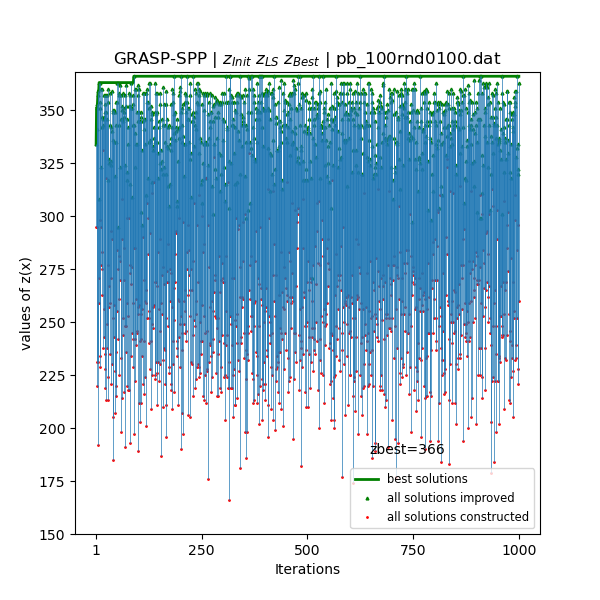
\includegraphics[width = .95\textwidth]{run00.png}}
  \only<2>{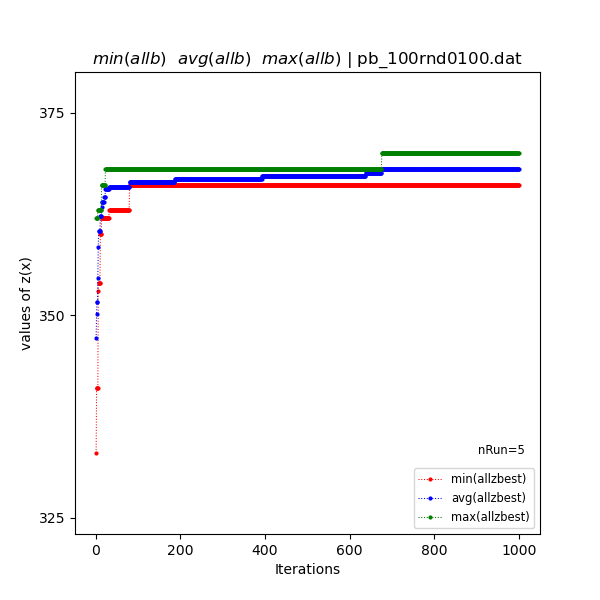
\includegraphics[width = .95\textwidth]{allruns00.png}}  
  
   $\alpha=0.00$
\end{column}
\begin{column}{0.55\textwidth}
\centering
    \only<1>{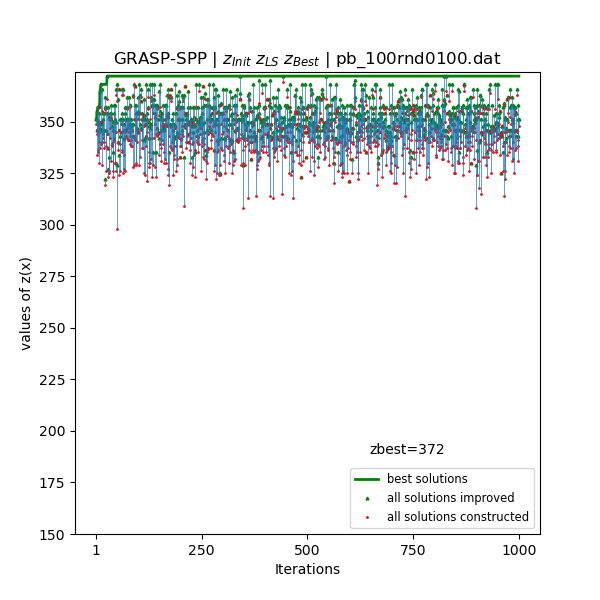
\includegraphics[width = .95\textwidth]{run07.png}}
    \only<2>{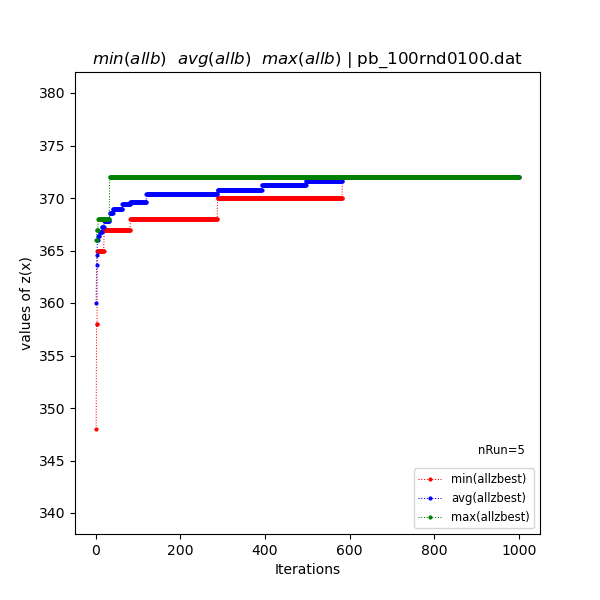
\includegraphics[width = .95\textwidth]{allruns07.png}}      
  
   $\alpha = 0.70$
\end{column}
\begin{column}{0.295\textwidth}
\centering
    \only<1>{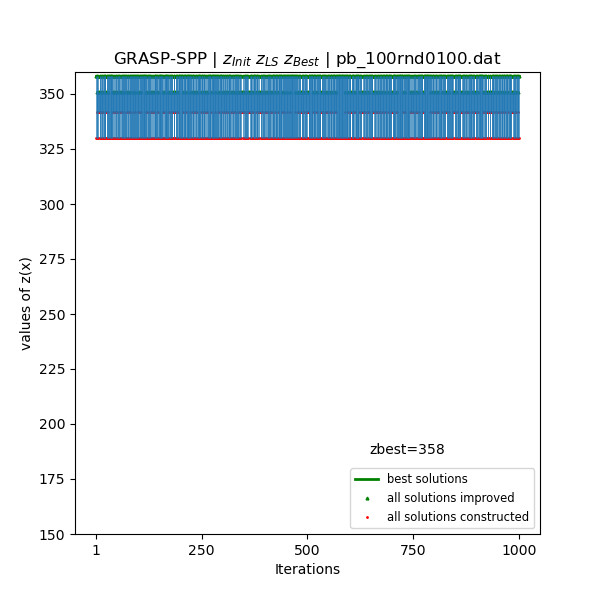
\includegraphics[width = .95\textwidth]{run10.png}}
    \only<2>{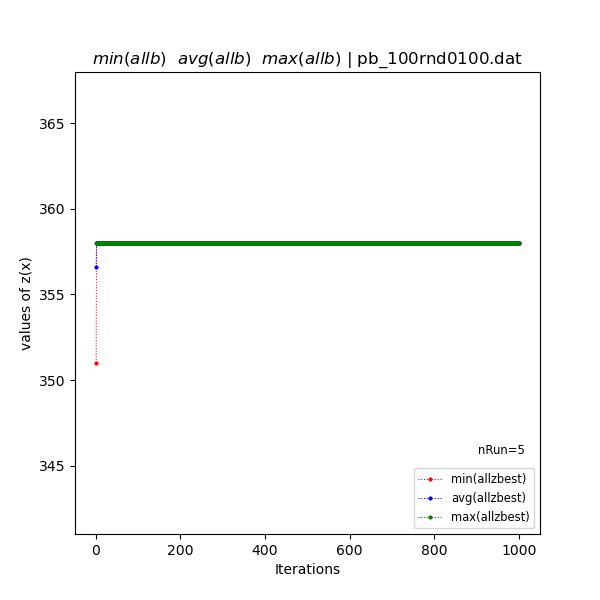
\includegraphics[width = .95\textwidth]{allruns10.png}}       
  
   $\alpha = 1.00$
\end{column}
\end{columns}

\end{frame}

% ================================================================
% ================================================================
% ================================================================

\begin{frame}[standout]

Topic 1

\end{frame}

% ================================================================
\begin{frame}{Topic 1}
\vspace{2mm}

\begin{columns}
\begin{column}{0.425\textwidth}
During MIC'1997, Sophia-Antipolis (France):
\vspace{4mm}

Private communication with Ibrahim Osman (American University of Beirut, Lebanon): 
\vspace{1mm}

\color{blue}adapting GRASP to MultiObjective Optimization\color{black}\\
\vspace{-2mm}

{\small 
\[
\begin{array}{clrclrrrl}
\min   & F(x)   \\
s.t.     & x  \ \in \ X
\end{array}
\]


\vspace{1mm}
\noindent 
where
%\vspace{2mm}
%\vfill
$
%
X \subseteq\mR^n, \
Y=F(X)\subseteq \mR^{\red{p}}
%
$
\color{blue}
\vspace{1.5mm}
to compute
$
%
X_{PE} \subset X, \
Y_{PN}\subset Y
%
$
\color{black}
}
\end{column}
\begin{column}{0.42\textwidth}
$\mbox{ }$\ \fbox{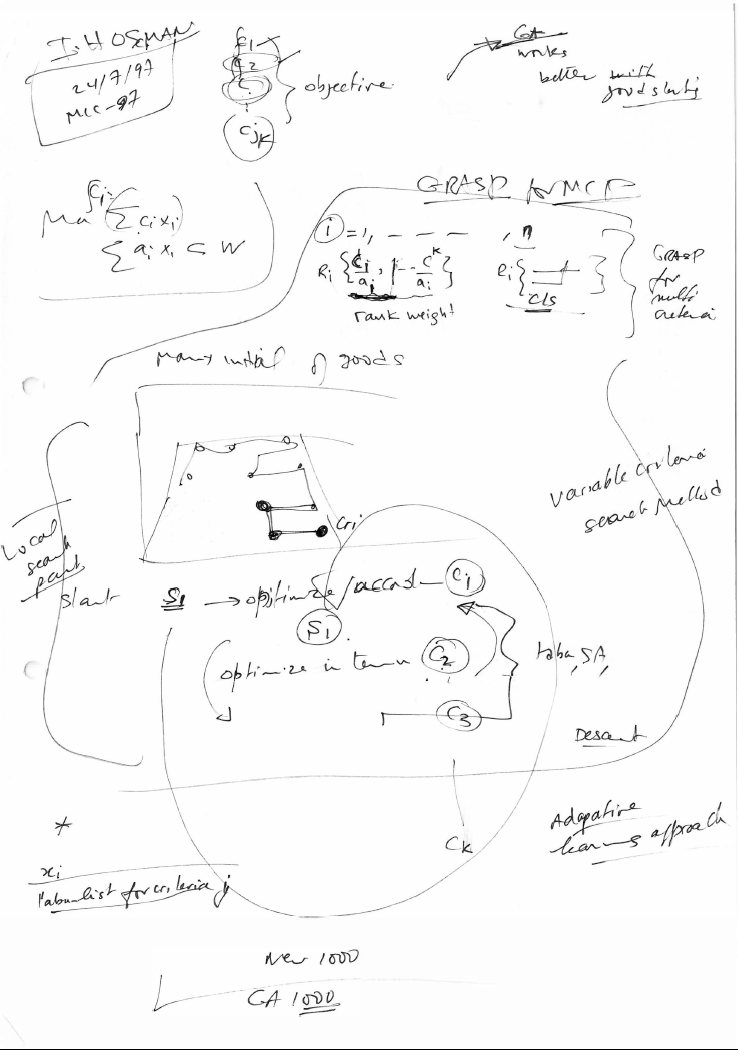
\includegraphics[scale=0.199]{relique1.png}}
\end{column}
\end{columns}

\end{frame}

% ================================================================
\begin{frame}{Topic 1}
\vspace{2mm}

\begin{columns}
\begin{column}{0.485\textwidth}
\hspace{-3mm}$\bullet$ Master thesis of D. Vancoppenolle
\vspace{2mm}

\onslide<2->{
\hspace{-3mm}$\bullet$ MCDM'1998 Charlotteville (USA):
\vspace{2mm}

{\tiny Xavier Gandibleux, David Vancoppenolle, Daniel Tuyttens, A first making use of GRASP for solving MOCO 
problems. MCDM'1998: 14th International Conference on Multiple Criteria Decision Making, June 8-12 1998, Charlottesville (VA), USA.

}
\vspace{4mm}
}

{\scriptsize
\color{blue}
$\circlearrowright d 
\left\{\begin{array}{lcc}
x_0 \leftarrow construction(\lambda^d) \\ 
x'_0 \leftarrow localSearch(x_0)\\
\circlearrowright  i
\left\{\begin{array}{lcc}
\only<1-2>{
x \leftarrow \color{blue} deconstruction\color{blue}(x'_{i-1})\\
x_i \leftarrow \color{blue} reconstruction\color{blue}(x, \lambda^d) \\
}
\only<3->{
x \leftarrow \color{purple} deconstruction\color{blue}(x'_{i-1})\\
x_i \leftarrow \color{purple} reconstruction\color{blue}(x, \lambda^d) \\
}
x'_i \leftarrow localSearch(x_i)\\
\end{array}\right.
\end{array}\right.
$
}
\vspace{4mm}

\only<1>{
\vspace{2mm}

$\mbox{ }$ 

\vspace{14mm}

}

\only<2>{
\vspace{2mm}

{\tiny Matthias Ehrgott, Xavier Gandibleux.
A survey and annotated bibliography of multiobjective combinatorial optimization. \textit{OR Spectrum}. 22(4): 425-460 (2000)

}
\vspace{6mm}

}

%\only<1>{\color{white} $\rightsquigarrow$ LNS (Shaw, 1998): \vspace{1.5mm}\\ {\scriptsize\textit{In LNS, an initial solution is gradually improved by alternately  destroying  and  repairing the solution} (Pisinger and Røpke 2010)\color{black}\\ } } 
\only<3>{$\rightsquigarrow$ \color{purple} LNS \color{black}(Shaw, 1998): \vspace{1.5mm}\\ {\scriptsize\textit{In LNS, an initial solution is gradually improved by alternately  \color{purple}destroying \color{black} and  \color{purple}repairing \color{black} the solution} (Pisinger and Røpke 2010)\\}}

\end{column}
\begin{column}{0.45\textwidth}
%\centering
\hspace{-6mm}
\only<1>{\fbox{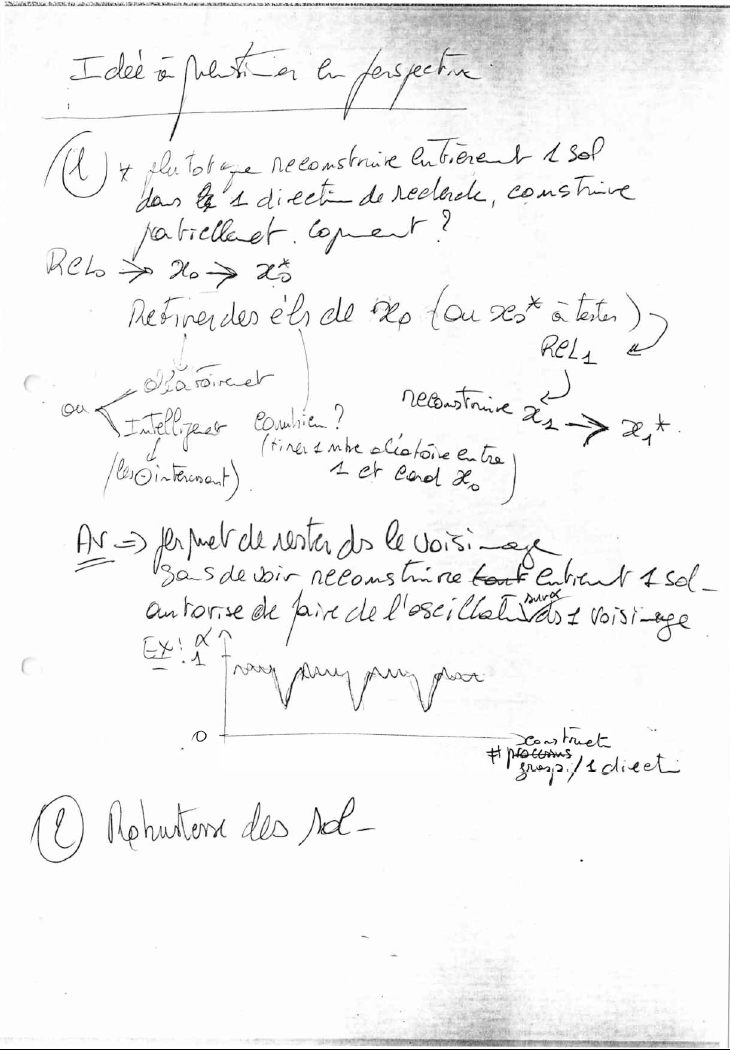
\includegraphics[scale=0.2]{relique2.png}}}
\only<2->{\hspace{2mm}\fbox{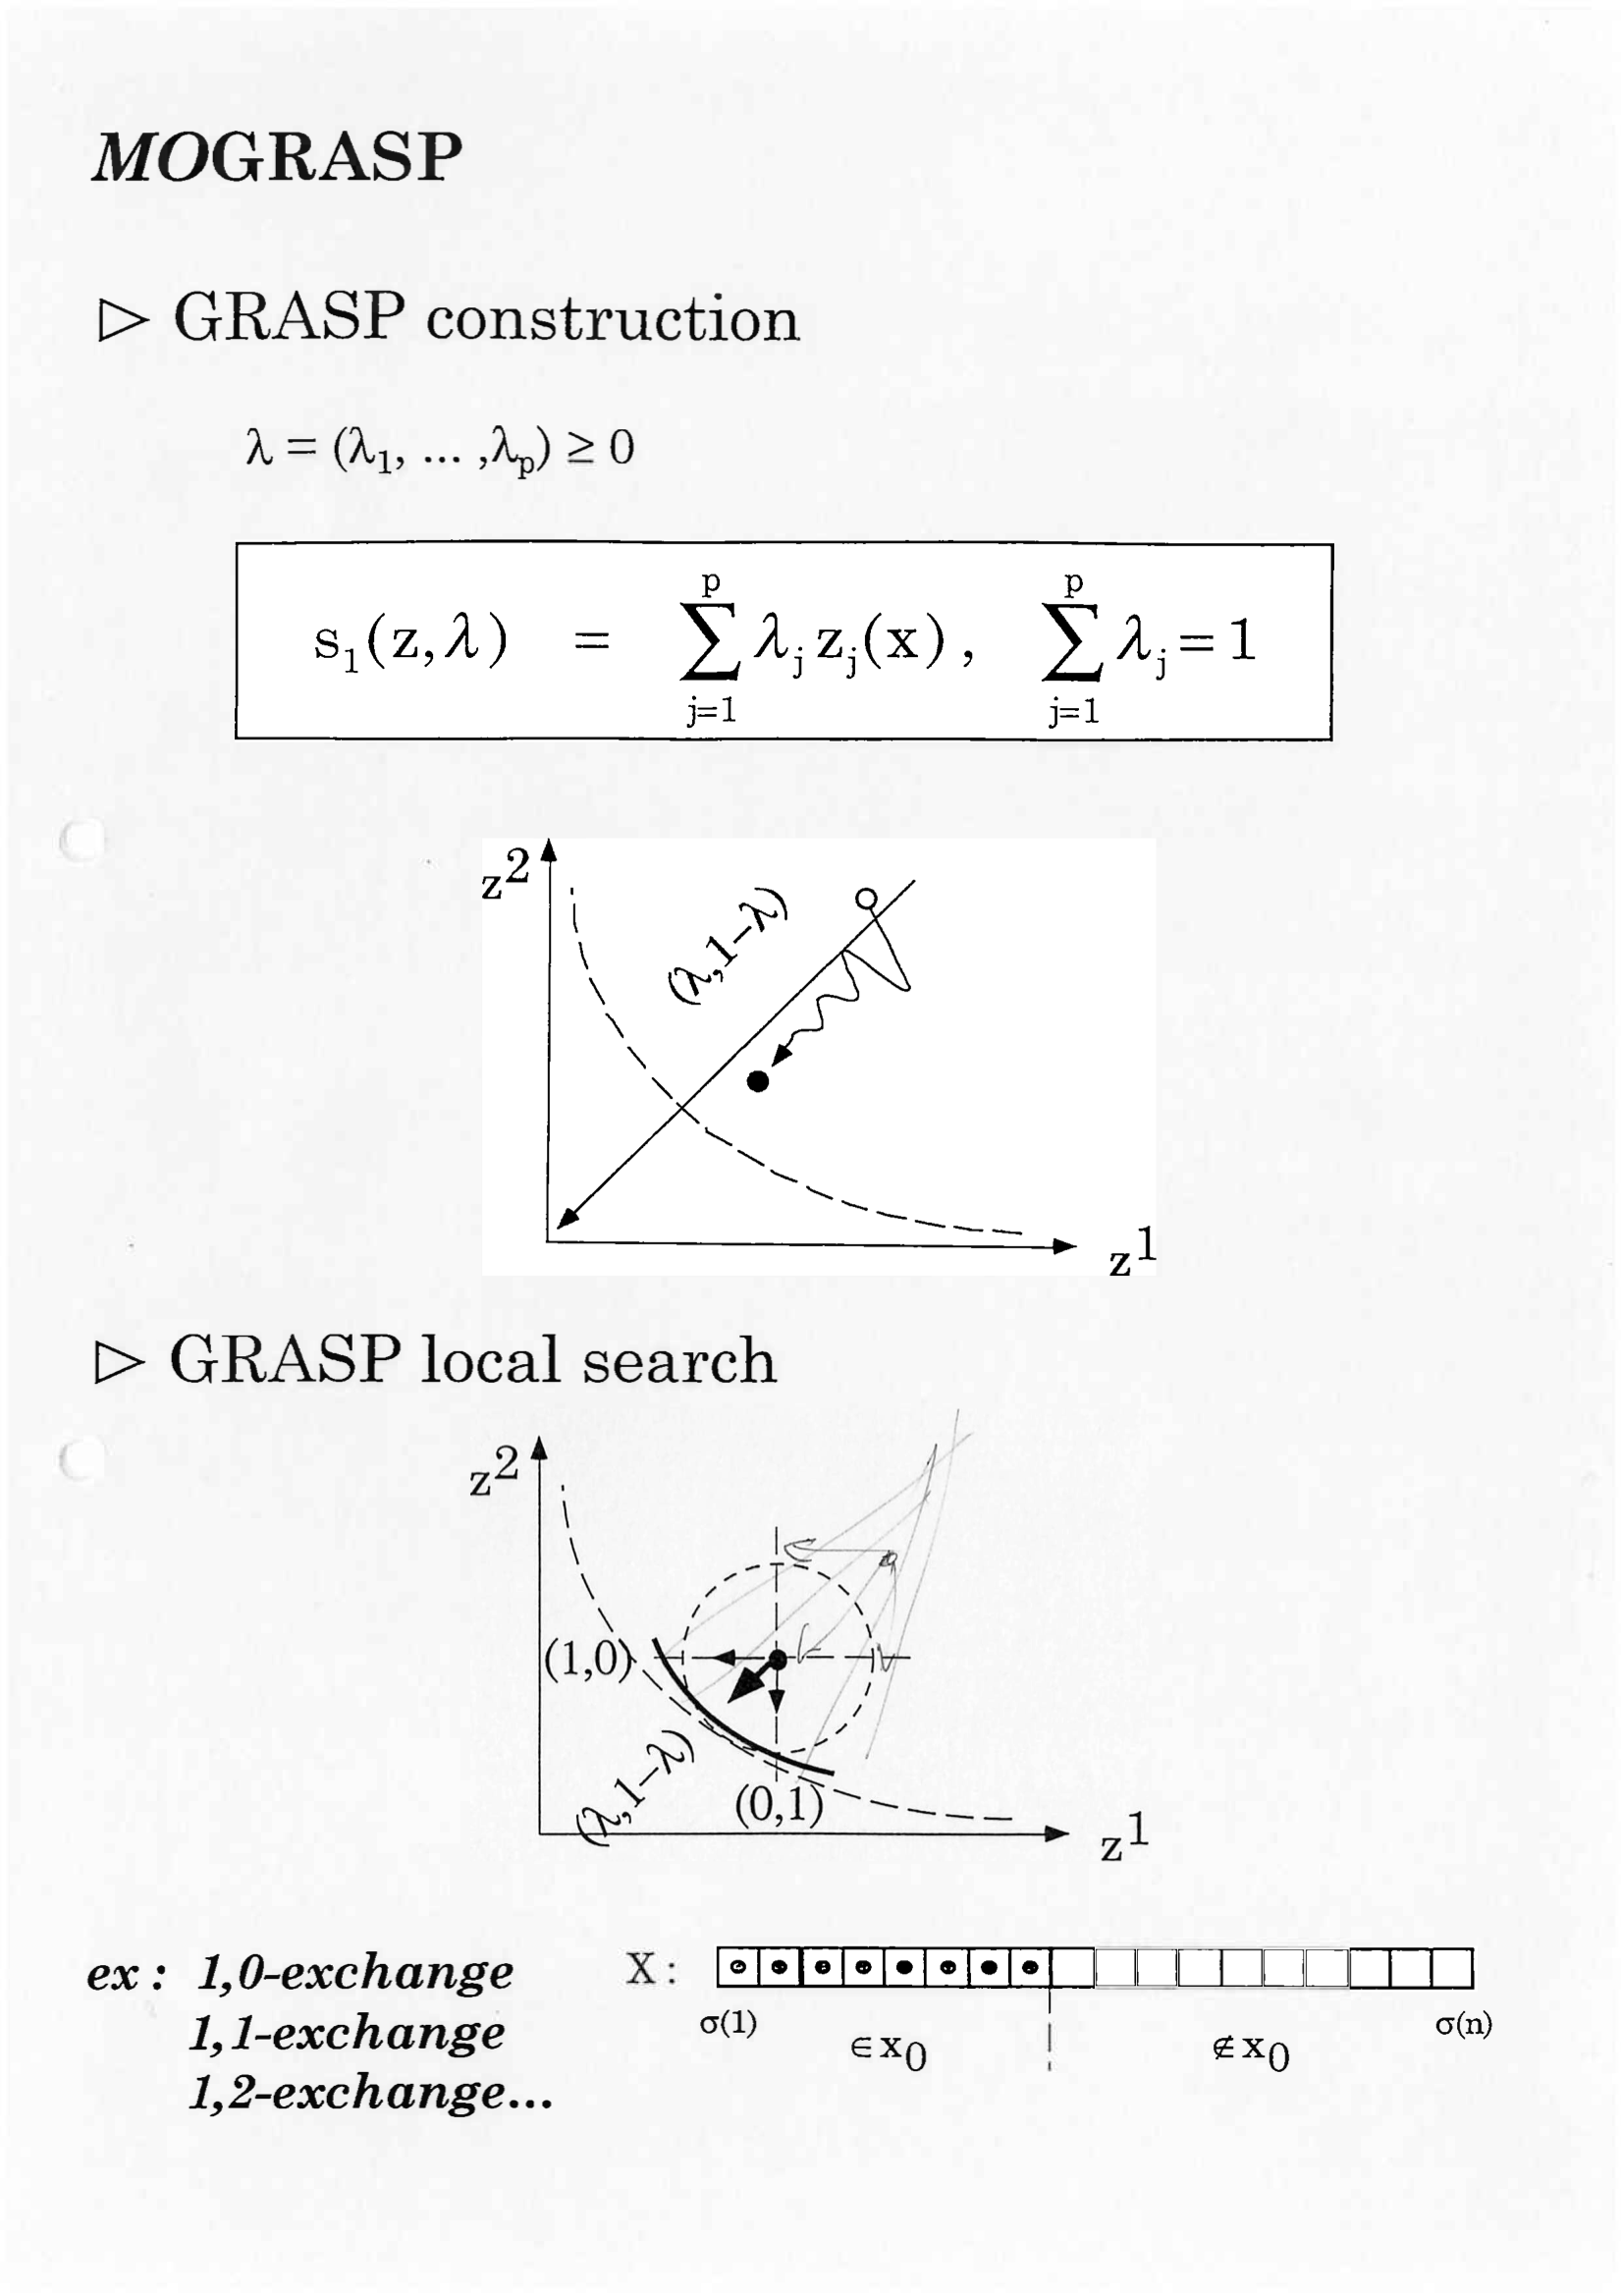
\includegraphics[scale=0.0875]{relique3.png}}}
\end{column}
\end{columns}

\end{frame}

% ================================================================
\begin{frame}{Topic 1}
\vspace{2mm}

Illustration (1-SPP): 
%\vspace{-1mm}

\begin{columns}
\begin{column}{0.5\textwidth}
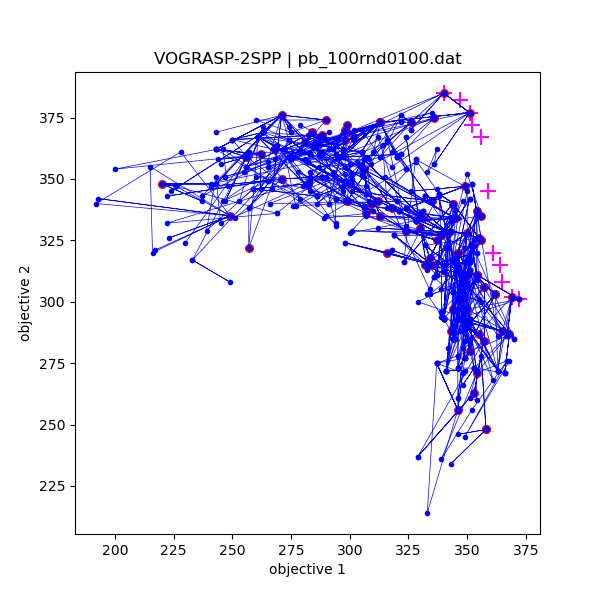
\includegraphics[scale=0.4]{VOGRASP100.png}
\end{column}
\begin{column}{0.5\textwidth}
 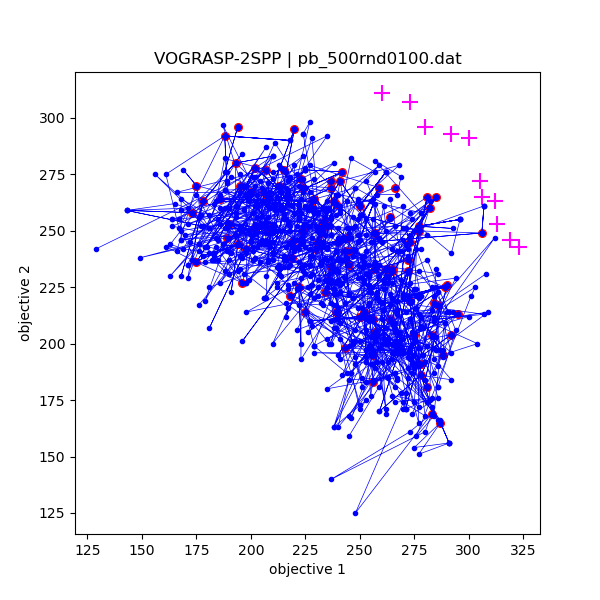
\includegraphics[scale=0.4]{VOGRASP500exact.png}
\end{column}
\end{columns}
\vspace{-2mm}

{\small 
\begin{itemize}
\item $\alpha$ = 0.7 \hfill value for computing U$_{limit}$ into RCL\vspace{-1mm}

\item nb$\lambda$ = 100 \hfill \# search directions from 0.0 to 1.0, step 0.01\vspace{-1mm}

\item nbDR = 15 \hfill \# deconstruction/reconstruction
\end{itemize}
} 

\end{frame}

%% ================================================================
%\begin{frame}{Topic 1}
%
%During MIC'1997, Sophia-Antipolis (France):
%
%\begin{itemize}
%
%\item[] Private communication with Ibrahim Osman (American University of Beirut, Lebanon): \color{blue}adapting GRASP to MultiObjective Optimization.\color{black}
%
%\end{itemize}
%\vspace{4mm}
%
%\begin{columns}
%\begin{column}{0.45\textwidth}
%\centering
%\fbox{
%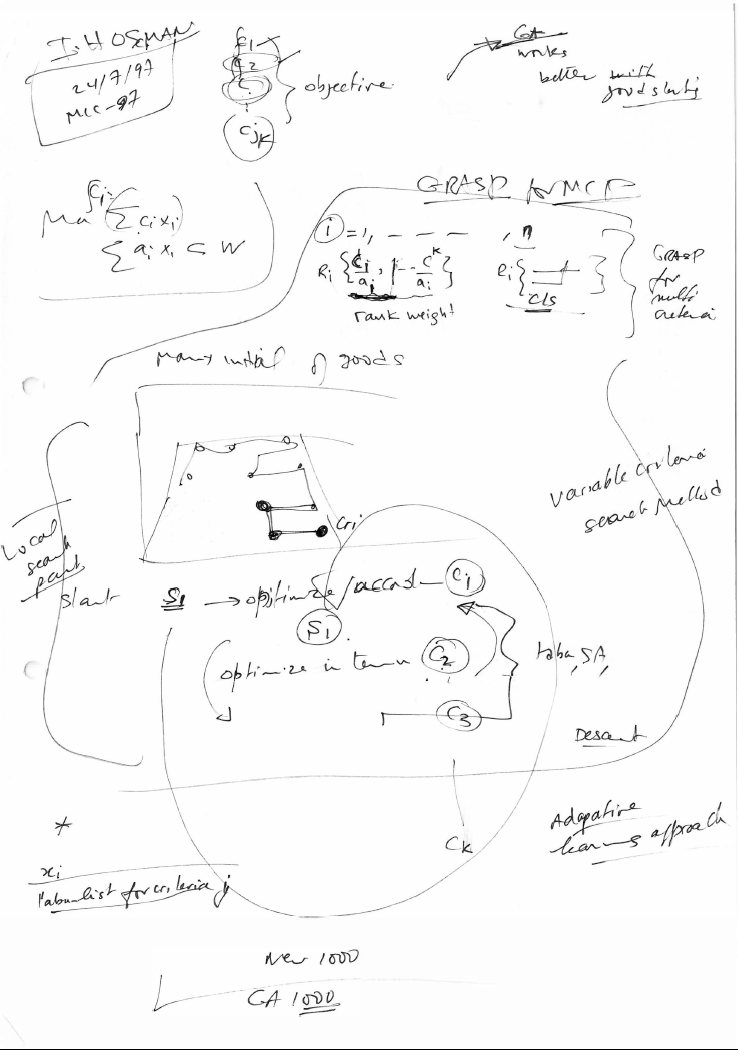
\includegraphics[scale=0.15]{relique1.png}
%}
%\end{column}
%\begin{column}{0.45\textwidth}
%\centering
%\fbox{
%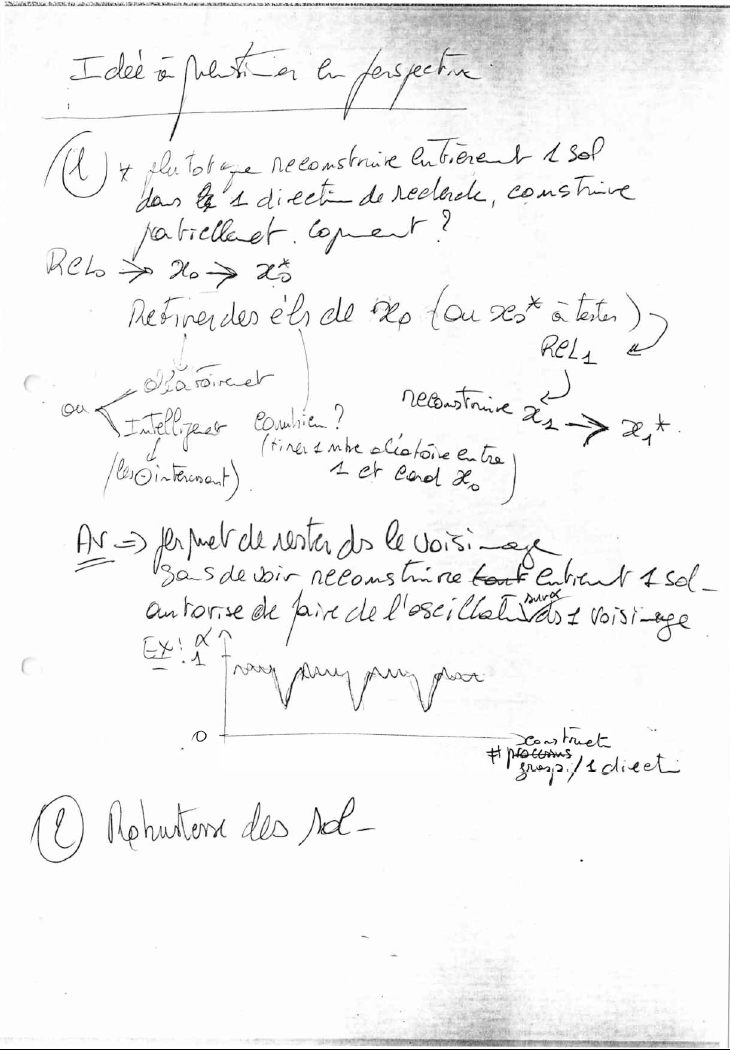
\includegraphics[scale=0.15]{relique2.png}
%}
%\end{column}
%\end{columns}
%
%%\only<1>{\includegraphics[scale=0.4]{ensBornants6.png}}
%
%\end{frame}

%% ================================================================
%\begin{frame}{Topic 1}
%
%Master thesis of D. Vancoppenolle,  MCDM'1998, Charlotteville (USA):
%
%\begin{columns}
%\begin{column}{0.05\textwidth}
%\end{column}
%\begin{column}{0.95\textwidth}
%\tiny{Xavier Gandibleux, David Vancoppenolle, Daniel Tuyttens, A first making use of GRASP for solving MOCO 
%problems. MCDM'1998: 14th International Conference on Multiple Criteria Decision Making, June 8-12 1998, Charlottesville (VA), USA.
%}
%\end{column}
%\end{columns}
%
%
%
%{\footnotesize
% for $d$ in 1:nDirections do\\
%\begin{enumerate}
%\item $x_0$ $\leftarrow$ GreedyRandomized construction for a convex combination $\lambda^d$ of objectives\\
%$x'_0$ $\leftarrow$ localSearch($x_0$)
%\item for $i$ in 1:nIter do\\
%\quad $x^{D}$ $\leftarrow$ destroy($x'_{i-1}$) with a RCL using $\beta$ worst candidates in $x'_{i-1}$\\
%\quad $x_i$ $\leftarrow$ reconstruct($x^{D}$) with a RCL using $\alpha$ best candidates for $\lambda^d$ \\
%\quad $x'_i$ $\leftarrow$ localSearch($x_i$)\\
%end \vspace{-4mm}
%\end{enumerate}
%end
%}

%$\rightsquigarrow$ LNS (Shaw, 1998)
%\end{frame}

% ================================================================
\begin{frame}{GRASP and multiObjective Optimization}

Examples of contributions :

{\scriptsize
\begin{itemize}
\item[2004:]
D. S. Vianna and J. E. C. Arroyo. A GRASP algorithm for the multi-objective knapsack problem.  \textit{XXIV International Conference of the Chilean Computer Science Society}, Arica, Chile, pp. 69-75.\vspace{1mm}\\

\item[2009:]
Li, H., Landa-Silva, D. (2009). An Elitist GRASP Metaheuristic for the Multi-objective Quadratic Assignment Problem. In: Ehrgott, M., Fonseca, C.M., Gandibleux, X., Hao, JK., Sevaux, M. (eds) Evolutionary Multi-Criterion Optimization. EMO 2009. \textit{Lecture Notes in Computer Science}, vol 5467. Springer, Berlin, Heidelberg. \vspace{1mm}\\

\item[2011:]
Arroyo, J.C., de Souza Pereira, A.A. A GRASP heuristic for the multi-objective permutation flowshop scheduling problem. \textit{The International Journal of Advanced Manufacturing Technology}.  55, 741–753.\vspace{1mm}\\

\item[2015:]
Rafael Martí, Vicente Campos, Mauricio G.C. Resende, Abraham Duarte,
Multiobjective GRASP with Path Relinking,
\textit{European Journal of Operational Research},
Volume 240, Issue 1, Pages 54-71.\vspace{1mm}\\

\item[2018:]
López-Sánchez, A.D., Hernández-Díaz, A.G., Gortázar, F. and Hinojosa, M.A., A multiobjective GRASP–VND algorithm to solve the waste collection problem. \textit{International Transactions in Operational Research}, 25(2): 545-567. 2018.\vspace{1mm}\\

\item[2021:]
Pedro Casas-Martínez, Alejandra Casado-Ceballos, Jesús Sánchez-Oro, and Eduardo G. Pardo. Multi-Objective GRASP for Maximizing Diversity. \textit{Electronics} 10(11):1232. 2021.\vspace{1mm}\\

\item[2022:]
Xing Wan, Zuo Xingquan, Li Xiaodong, and Zhao Xinchao. A Hybrid Multiobjective GRASP for a Multi-Row Facility Layout Problem with Extra Clearances. \textit{International Journal of Production Research} 60(3), 957–976. 2022.\\
\end{itemize}
}

\end{frame}

% ================================================================
\begin{frame}[fragile]{GRASP and deconstruction/reconstruction}

GRASP $\approx$ LNS with 100\% of deconstruction.
\bigskip

Investigation on 1-objective Weighted Set Packing Problem (1-WSPP): 

\begin{itemize} 
\item Valentin Antuori (2014): \\ GRASP\_DR v.s. LNS

\item Elizabeth Gandibleux and Awen Jacq-Bodet (2023): \\  GRASP\_DR := GRASP + DR[rnd/VND]
\end{itemize}
\bigskip

Deconstruction (randomly):\\
\begin{itemize}
\item identify the \texttt{nList1} variables at 1 into $x'_0$
\item remove 33\% $\le$ rand(1:nList1) $\le$ 50\% of   variables at 1 into $x'_0$
\end{itemize}

Reconstruction (following VND principle):\\
\begin{itemize}
\item 0-1 exchange $ \longrightarrow$
 1-1 exchange $ \longrightarrow$
 2-1 exchange
\end{itemize}

\end{frame}

% ================================================================
\begin{frame}[fragile]{GRASP and deconstruction/reconstruction}
1-WSPP $\mid$ Nb instances : 65 $\mid$ example of 1 run :
\begin{columns}
\begin{column}{0.9\textwidth}
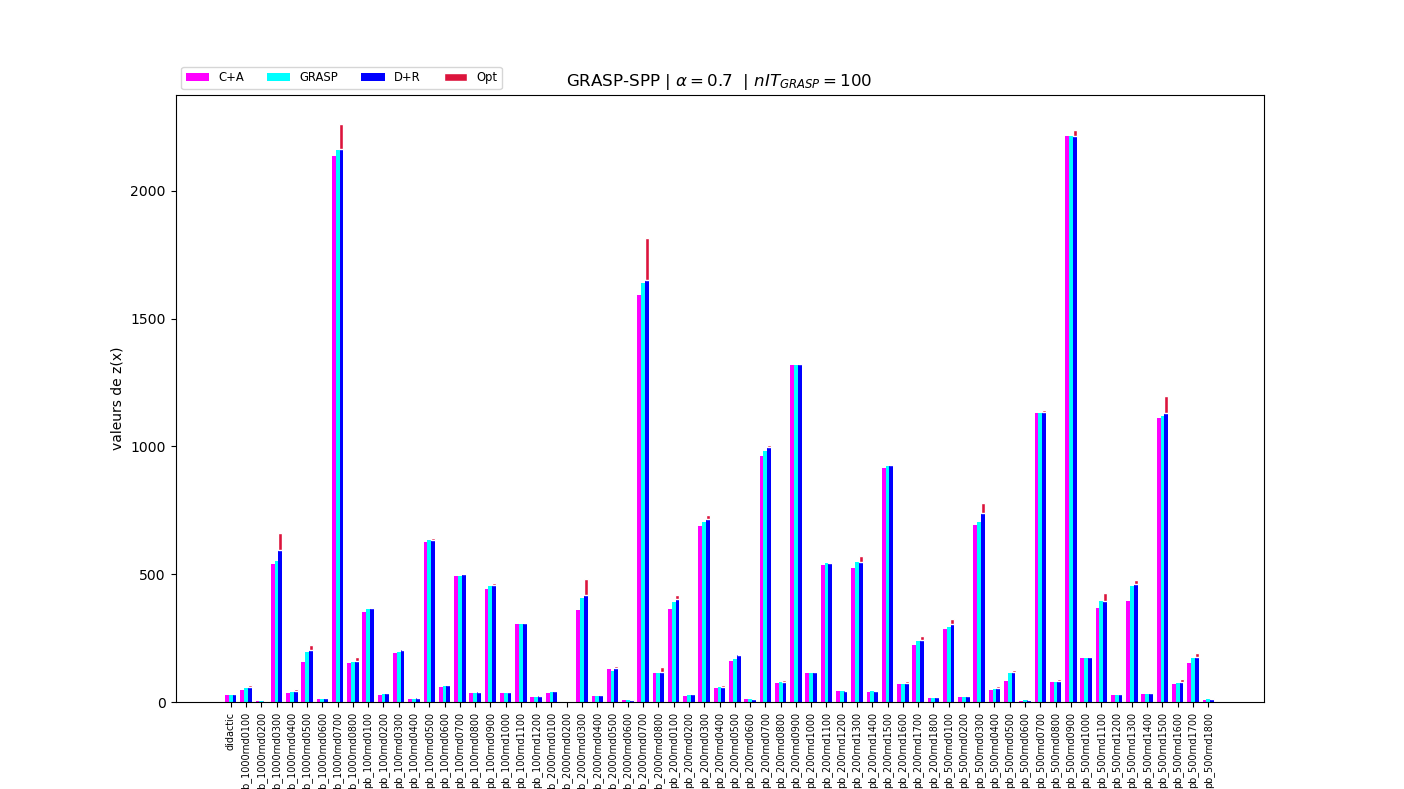
\includegraphics[scale=0.375]{GRASPDR.png}
\end{column}
\begin{column}{0.5\textwidth}
\end{column}
\end{columns}
\end{frame}

% ================================================================
\begin{frame}{GRASP and deconstruction/reconstruction}

   1 run with 
    $\alpha$       = 0.70  $\mid$
    nbIterGrasp = 100 $\mid$
    nbIterDR     = 10  $\mid$
    bests :

{\scriptsize
\begin{center}
\begin{tabular}{|c|c|c|c|c|r|c|c|}
\hline
instance & C+A & GRASP & GRASP\_DR  & bestKnown\\
\hline
 100rnd0100 & 351 & 368 & \textbf{370} & 372  \\
 100rnd0200 & 29 & 32 & \textbf{33} & 34    \\
 100rnd0300 & 194 & 195 & \textbf{203} & 203   \\
 100rnd0400 & 13 & \textbf{15} & \textbf{15} & 16    \\
% 100rnd0500 & 627 & 633 & 633 & 633  &      GRASP  GRASP\_DR  \\
% 100rnd0600 & 61 & 64 & 64 & 64 &      GRASP  GRASP\_DR  \\
% 100rnd0700 & 495 & 495 & 499 & 499  &      GRASP\_DR  \\
% 100rnd0800 & 37 & 37 & 38 & 38  &      GRASP\_DR  \\
% 100rnd0900 & 442 & 453 & 456 & 456  &      GRASP\_DR  \\
% 100rnd1000 & 36 & 38 & 39 & 39  &      GRASP\_DR  \\
% 100rnd1100 & 306 & 306 & 306 & 306  &      C+A  GRASP  GRASP\_DR  \\
% 100rnd1200 & 21 & 22 & 23 & 23  &      GRASP\_DR  \\
\hline
 200rnd0100 & 366 & 400 & \textbf{415} & 416   \\
 200rnd0200 & 25 & 29 & \textbf{30} & 32   \\
 200rnd0300 & 689 & \textbf{721} & \textbf{721} & 731   \\
 200rnd0400 & 55 & 58 & \textbf{60} & 64    \\
% 200rnd0500 & 162 & 170 & 184 & 184  &      GRASP\_DR  \\
% 200rnd0600 & 11 & 12 & 13 & 13  &      GRASP\_DR  \\
% 200rnd0700 & 961 &  994 & 995 & 995  &      GRASP\_DR  \\
% 200rnd0800 & 75 & 80 & 81 & 81  &      GRASP\_DR  \\
% 200rnd0900 & 1319 & 1324 & 1324 & 1324  &      GRASP  GRASP\_DR  \\
% 200rnd1000 & 115 & 16 & 117 & 117  &      GRASP\_DR  \\
% 200rnd1100 & 536 & 544 & 544 & 544 &      GRASP  GRASP\_DR  \\
% 200rnd1200 & 42 & 42 & 43 & 43  &      GRASP\_DR  \\
% 200rnd1300 & 525 & 551 & 557 & 557  &      GRASP\_DR  \\
% 200rnd1400 & 39 & 43 & 44 & 44  &      GRASP\_DR  \\
% 200rnd1500 & 915 & 926 & 926 & 926  &      GRASP  GRASP\_DR  \\
% 200rnd1600 & 70 & 72 & 75 & 75  &      GRASP\_DR  \\
% 200rnd1700 & 223 & 239 & 255 & 255  &      GRASP\_DR  \\
% 200rnd1800 & 15 & 18 & 18 & 18  &      GRASP  GRASP\_DR  \\
\hline
 500rnd0100 & 285 & 309 & \textbf{312} & 323    \\
 500rnd0200 & 19 & 21 & \textbf{22} & 25    \\
 500rnd0300 & 694 & 724 & \textbf{749} & 776    \\
 500rnd0400 & 47 & 54 & \textbf{55} & 62   \\
% 500rnd0500 & 84 & 118 & 118 & 118  &      GRASP  GRASP\_DR  \\
% 500rnd0600 & 6 & 7 & 8 & 8  &      GRASP\_DR  \\
% 500rnd0700 & 1131 & 1141 & 1141 & 1141  &      GRASP  GRASP\_DR  \\
% 500rnd0800 & 78 & 81 & 83 & 83  &      GRASP\_DR  \\
% 500rnd0900 & 2212 & 2225 & 2221 & 2225  &      GRASP  \\
% 500rnd1000 & 171 & 174 & 174 & 174  &      GRASP  GRASP\_DR  \\
% 500rnd1100 & 367 & 394 & 412 & 412  &      GRASP\_DR  \\
% 500rnd1200 & 28 & 31 & 30 & 31  &      GRASP  \\
% 500rnd1300 & 397 & 453 & 460 & 460  &      GRASP\_DR  \\
% 500rnd1400 & 31 & 34 & 36 & 36  &      GRASP\_DR  \\
% 500rnd1500 & 1112 & 1145 & 1166 & 1166  &      GRASP\_DR  \\
% 500rnd1600 & 72 & 77 & 80 & 80  &      GRASP\_DR  \\
% 500rnd1700 & 154 & 175 & 186 & 186  &      GRASP\_DR  \\
% 500rnd1800 & 9 & 12 & 13 & 13  &      GRASP\_DR  \\
\hline
 1000rnd0100 & 49 & \textbf{67} & \textbf{67} & 67    \\
 1000rnd0200 & \textbf{3} & \textbf{3} & \textbf{3} & 4    \\
 1000rnd0300 & 541 & 582 & \textbf{592} & 661    \\
 1000rnd0400 & 37 & \textbf{43} & \textbf{43} & 48    \\
% 1000rnd0500 & 157 & 214 & 214 & 214  &      GRASP  GRASP\_DR  \\
% 1000rnd0600 & 11 & 13 & 13 & 13  &      GRASP  GRASP\_DR  \\
% 1000rnd0700 & 2136 & 2176 & 2191 & 2191  &      GRASP\_DR  \\
% 1000rnd0800 & 154 & 161 & 158 & 161  &      GRASP  \\
\hline
 2000rnd0100 & 37 & \textbf{40} & \textbf{40} & 40    \\
 2000rnd0200 & \textbf{2} & \textbf{2} & \textbf{2} & 2    \\
 2000rnd0300 & 361 & 428 & \textbf{434} & 478    \\
 2000rnd0400 & 25 & 26 & \textbf{28} & 32    \\
 %2000rnd0500 & 128 & 140 & 140 & 140  &      GRASP  GRASP\_DR  \\
% 2000rnd0600 & 7 & 9 & 9  &      GRASP  GRASP\_DR  \\
% 2000rnd0700 & 1592 & 1693 & 1693 & 1693  &      GRASP  GRASP\_DR  \\
% 2000rnd0800 & 113 & 116 & 117 & 117  &      GRASP\_DR  \\
\hline
\end{tabular}
\end{center}
}

Nb instances : 65; \#best:  C+A : 4 $\mid$ GRASP : 26 $\mid$ GRASP\_DR : 62

\end{frame}

% ================================================================
% ================================================================
% ================================================================

\begin{frame}[standout]

Topic 2

\end{frame}

% ================================================================
\begin{frame}{Topic 2}

During EURO'1997, Barcelona (Spain):

\begin{itemize}

\item Private communication with Naoki Katoh (Kyoto University, Japan) and Hiroyuki Morita (Osaka Prefecture University, Japan): 
\color{blue}strenghten EMO with LS for MOCO problems.\color{black}
\vspace{3mm}

$\drsh$ concept of seeding solutions in a EMO


{\tiny Hiroyuki Morita, Xavier Gandibleux, and Naoki Katoh. 
Experimental feedback on biobjective permutation scheduling problems solved with a population heuristic. 
\textit{Foundations of Computing and Decision Sciences Journal}. 26(1):23–50, 2001.

}
\vspace{3mm}

$\drsh$ seeding solutions generated with $\lambda$-GRASP


{\tiny Xavier Delorme, Xavier Gandibleux, and Fabien Degoutin. 
Evolutionary, constructive and hybrid procedures for the bi-objective set packing problem. 
\textit{European Journal of Operational Research}. 204(2):206–217, July 2010.

}
\vspace{3mm}

$\drsh$ methodology for MOMH  in 3 stages


{\tiny Xavier Gandibleux:
Peek - Shape - Grab: A Methodology in Three Stages for Approximating the Non-dominated Points of Multiobjective Discrete/Combinatorial Optimization Problems with a Multiobjective Metaheuristic. In: Trautmann, H., et al. Evolutionary Multi-Criterion Optimization. EMO 2017. Lecture Notes in Computer Science, vol 10173, 221-235. Springer. 2017.

}
\vspace{3mm}

\hfill ...visual demonstration...

\end{itemize}

\end{frame}

% ================================================================
\begin{frame}{Topic 2}

\centering
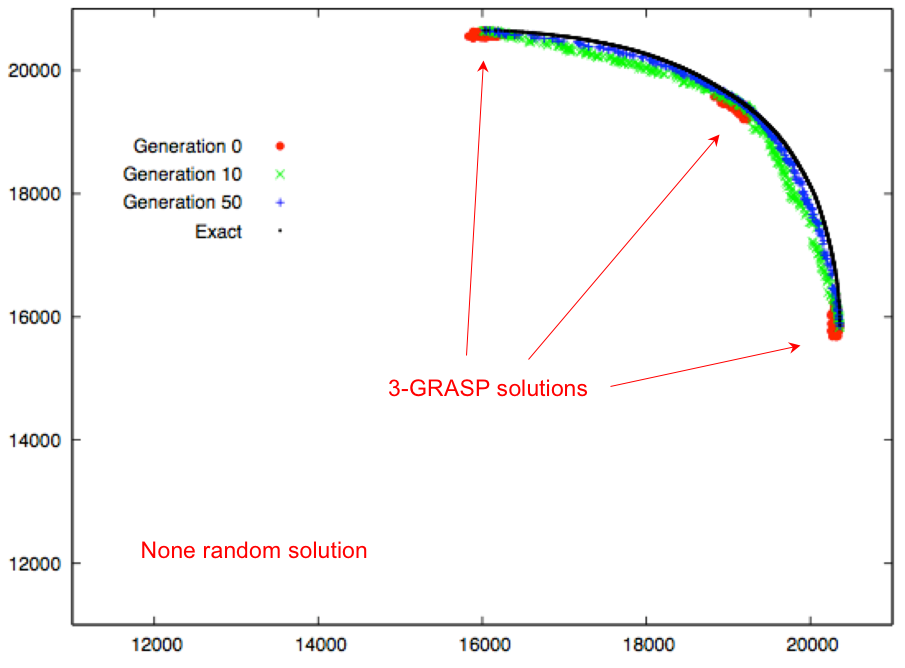
\includegraphics[scale=0.2]{lambdaGRASP.png}
\vspace{3mm}

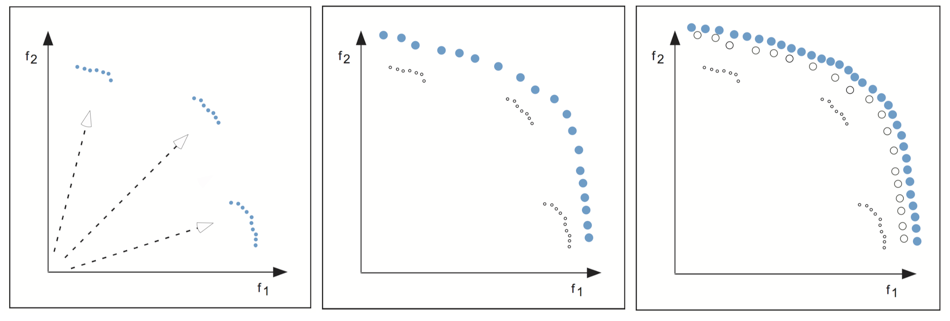
\includegraphics[scale=0.25]{psg.png}

\end{frame}


% ================================================================
\begin{frame}{MOMH using seeding solutions}


Examples of contributions :

{\scriptsize
\begin{itemize}

\item[2005:]     Christian Haubelt, Jürgen Gamenik, and Jürgen Teich . Initial population construction for convergence improvement of MOEAs. In Carlos Coello Coello, Arturo Hernandez Aguirre, and Eckart Zitzler, editors, Evolutionary Multi-Criterion Optimization. \textit{Lecture Notes in Computer Sciences}, volume 3410, pages 191–205. Springer Verlag, Berlin, Germany, 2005.\vspace{1mm}\\

\item[2009:] Sophie N. Parragh, Karl F. Doerner, Richard F. Hartl, Xavier Gandibleux.
A heuristic two-phase solution approach for the multi-objective dial-a-ride problem.
\textit{Networks}. 54: 227-242. 2009.\vspace{1mm}\\

\item[2018:]
Ana D. López-Sánchez, Alfredo G. Hernández-Díaz, Francisco Gortázar, and Miguel Hinojosa, 
A multiobjective GRASP–VND algorithm to solve the waste collection problem. \textit{International Transactions in Operational Research}. 25(2): 545-567. 2018.\vspace{1mm}\\

\item[2020:]
Takfarinas Saber, Xavier Gandibleux, Michael O'Neill, Liam Murphy, Anthony Ventresque.
A comparative study of multi-objective machine reassignment algorithms for data centres. 
\textit{Journal of Heuristics}. 26(1): 119-150, 2020.\vspace{1mm}\\

\item[2021:]
Ana. D. López-Sánchez, Jesus. Sánchez-Oro, Manuel Laguna. A New Scatter Search Design for Multiobjective Combinatorial Optimization with an Application to Facility Location. \textit{INFORMS Journal on Computing} 33(2):629-642. 2021.\vspace{1mm}\\

\item[2022:]
Yu Xue, Xu Cai, Ferrante Neri,
A multi-objective evolutionary algorithm with interval based initialization and self-adaptive crossover operator for large-scale feature selection in classification,
\textit{Applied Soft Computing}, Volume 127, 2022.\vspace{1mm}\\

\end{itemize}
}

\end{frame}

% ================================================================
% ================================================================
% ================================================================

\begin{frame}[standout]

Topic 3

\end{frame}

% ================================================================
\begin{frame}{Topic 3}

ReactiveGRASP: component to automatize the tuning of $\alpha$

{\tiny Marcelo Prais, Celso C. Ribeiro. Reactive GRASP:An application to a matrix decomposition problem in TDMA traffic assignment.
\textit{INFORMS Journal on Computing}. 12, 164-176. 2000.

}


\begin{itemize}
\item $n$ classes of probabilities, each class is associated to one value $\alpha$ 
\item $N_\alpha$ iterations before to update the probabilities
\end{itemize}

\only<1>{\vspace{0mm}
\vspace{13mm}

{\tiny Xavier Delorme, Xavier Gandibleux, Joaquin Rodriguez. GRASP for set packing problems. 
\textit{European Journal of Operational Research}. Volume 153, Issue 3, 2004.

}


Refactoring my material for my lecture about GRASP...

\vspace{3mm}

\hfill ...elaborated in 2019 a script drawing the evolution of probabilities...
\vspace{50mm}}
\only<2>{
\vspace{0mm}
%Observation on 1-objective Weighted Set Packing Problem (1-WSPP): 
\begin{columns}
\begin{column}{0.575\textwidth}
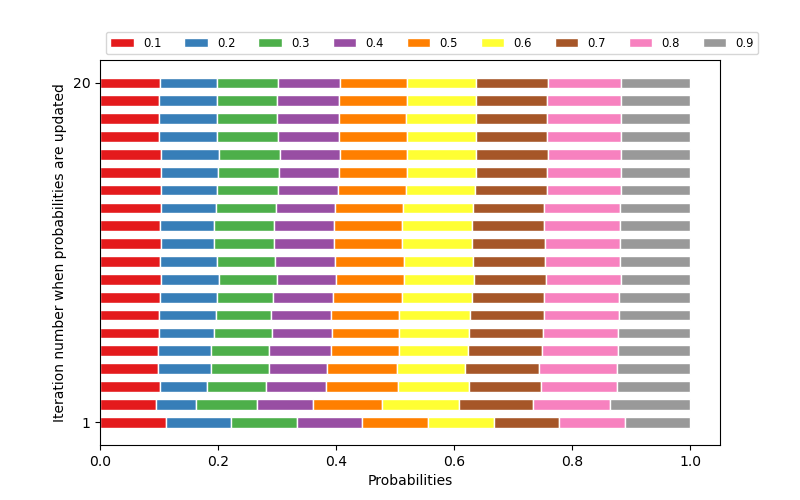
\includegraphics[scale=0.35]{GR1runalpha.png}
\end{column}
\begin{column}{0.45\textwidth}
 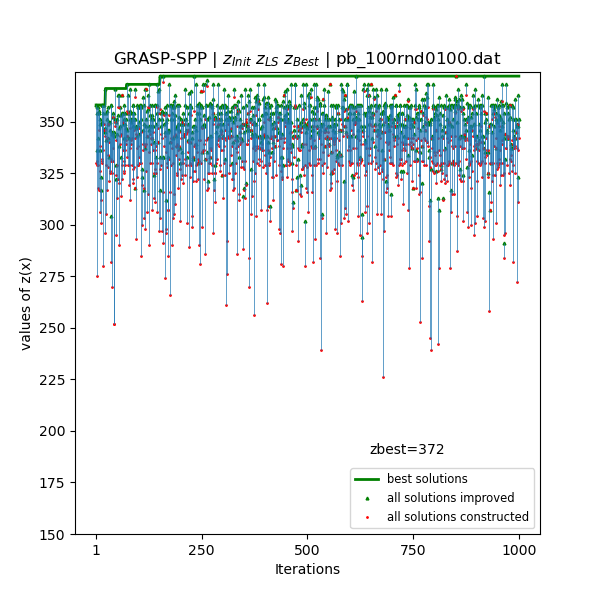
\includegraphics[scale=0.3]{GR1runz.png}
\end{column}
\end{columns}

\color{black} - no literature examining in detail the ``Reactive'' component\vspace{-1mm}\\ \ \ (private communication with Celso Ribeiro)\\
- same on 1-StPP, 1-TSP (Athanael Jousselin, Axel Verneuil, 2024)\\
\hfill \color{black}
}
\end{frame}

% ================================================================
\begin{frame}{Topic 3}



Tentative 1:
\begin{itemize} 
\item 2019: Amplify the changes on probabilities: \\  tested on 1-WSPP
\end{itemize}
\begin{columns}
\begin{column}{0.575\textwidth}
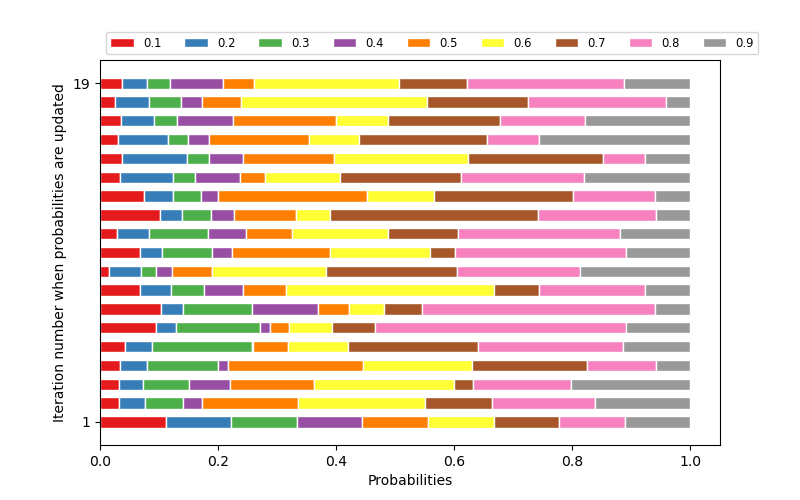
\includegraphics[scale=0.35]{arunalpha2019.png}
\end{column}
\begin{column}{0.45\textwidth}
 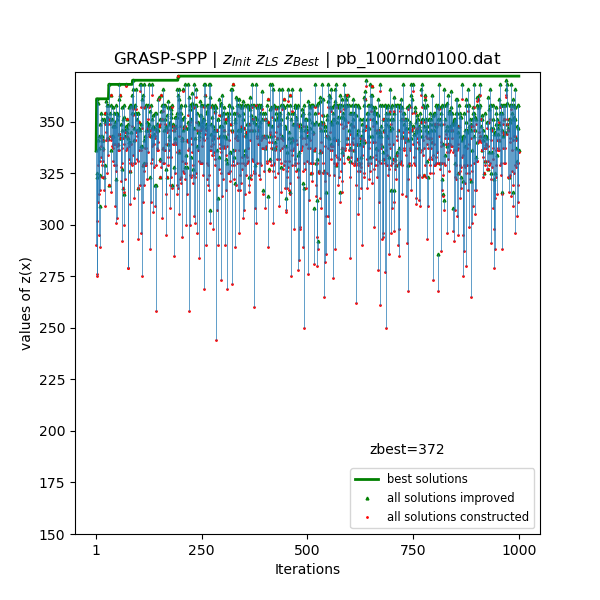
\includegraphics[scale=0.3]{arunz2019.png}
\end{column}
\end{columns}

\vfill

\end{frame}

%% ================================================================
%\begin{frame}{Topic 3}
%
%
%Tentative 2:
%\begin{itemize} 
%\item 2024: Athanael Jousselin, Axel Verneuil with Celso Ribeiro: \\  3 strategies on 1-WSPP, 1-StPP, 1-TSP
%\end{itemize}
%
%Blocking during some iterations the value of an improved probability
%
%Blocking  the value of an improved probability greater than a threshold
%
%Uniform distribution (computation budget distributed across all classes)
%
%\vfill
%
%
%\end{frame}

% ================================================================
\begin{frame}{Topic 3}


Tentative 2:
\begin{itemize} 
\item 2024: tentative 1 + freezing iteratively one class (i.e. $p_i \ge p_i^{min}$): \\   
$\drsh$  ReactiveGRASP strengthened, tested on 1-WSPP
\end{itemize}

Sketch:

$\circ$ parameters:\vspace{-3mm}
{\small
\begin{itemize}
\item \#classes + value $\alpha$ associated to each class\vspace{-1mm}
\item \#iterations GRASP to perform (init, search)
\end{itemize}
}

$\circ$ steps:  \vspace{-3mm}
{\small
\begin{enumerate}
\item [] ReactiveGRASP (Prais, Ribeiro 2000) +\vspace{-1mm}
\item initialize each class, set $N_\alpha$ according \#classes and \#iterations\vspace{-1mm}
\item acceptance threshold for updating the classes; automatically maintained\vspace{-1mm}
\item amplification mechanism;  distort probabilities for valuable classes visited\vspace{-1mm}
\item freezing mechanism; prevent the probability decrease of a good class
\end{enumerate}
}

$\Rightarrow$ after $N_\alpha$ iterations, at most 1 class is frozen


\vfill

\end{frame}

% ================================================================
\begin{frame}{Topic 3}

\textbf{\texttt{pb\_100rnd\_0100}} (100 variables; 500 constraints; density: 2\%; max1: 2)\\
z=372 (optimal)
\vspace{1mm}

1000 iterations:
\vspace{1mm}

\begin{columns}
\begin{column}{0.575\textwidth}
\centering
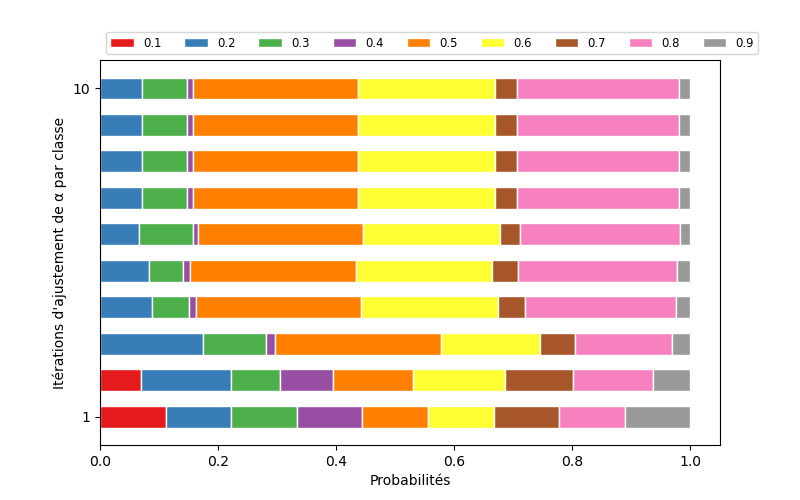
\includegraphics[scale=0.35]{proba100_100.png}

1 run
\end{column}
\begin{column}{0.45\textwidth}
\centering
 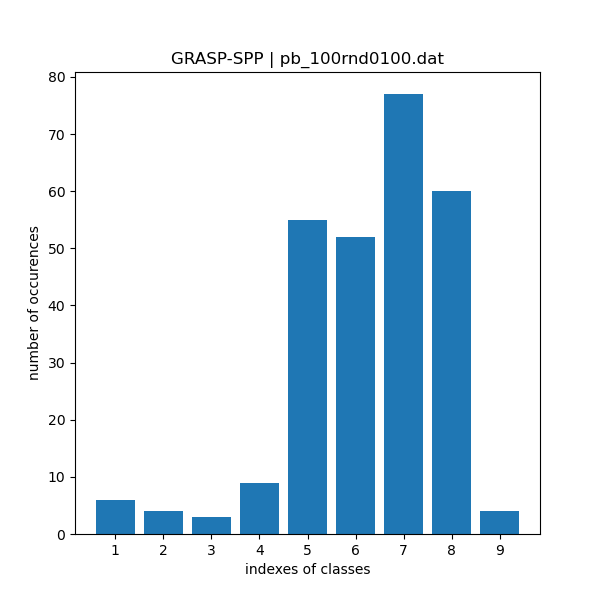
\includegraphics[scale=0.3]{all100_100.png}
 
 30 runs
\end{column}
\end{columns}

{\tiny
$z$: 
[372, 372, 372, 372, 372, 372, 372, 372, 372, 372, 372, 372, 372, 372, 372, 372, 372, 372, 372, 372, 372, 372, 372, 372, 372, 372, 372, 372, 372, 372]\vspace{1mm}\\
$\Delta$(\%): 
[0.0, 0.0, 0.0, 0.0, 0.0, 0.0, 0.0, 0.0, 0.0, 0.0, 0.0, 0.0, 0.0, 0.0, 0.0, 0.0, 0.0, 0.0, 0.0, 0.0, 0.0, 0.0, 0.0, 0.0, 0.0, 0.0, 0.0, 0.0, 0.0, 0.0]\\
}

\end{frame}

% ================================================================
\begin{frame}{Topic 3}

\textbf{\texttt{pb\_2000rnd\_0700}} (2000 vars; 2000 consts; density: 0.56\%; max1: 20)\\
z=1811 (best)
\vspace{1mm}

1000 iterations:
\vspace{1mm}


\begin{columns}
\begin{column}{0.575\textwidth}
\centering
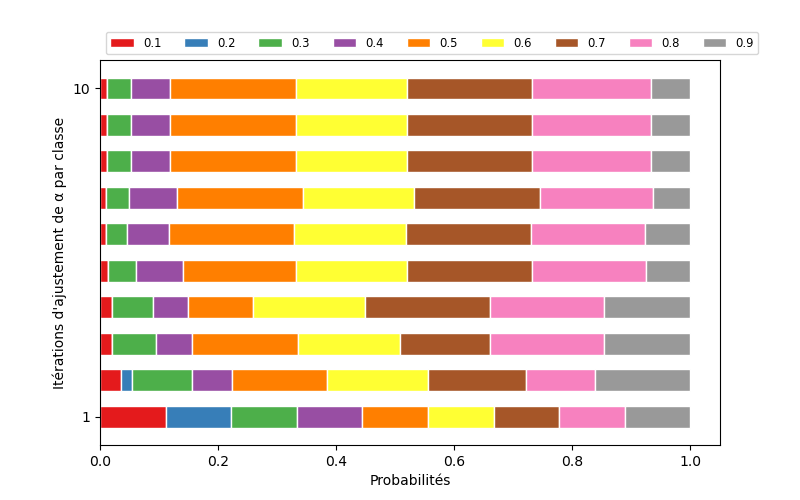
\includegraphics[scale=0.35]{proba2000_700.png}

1 run
\end{column}
\begin{column}{0.45\textwidth}
\centering
 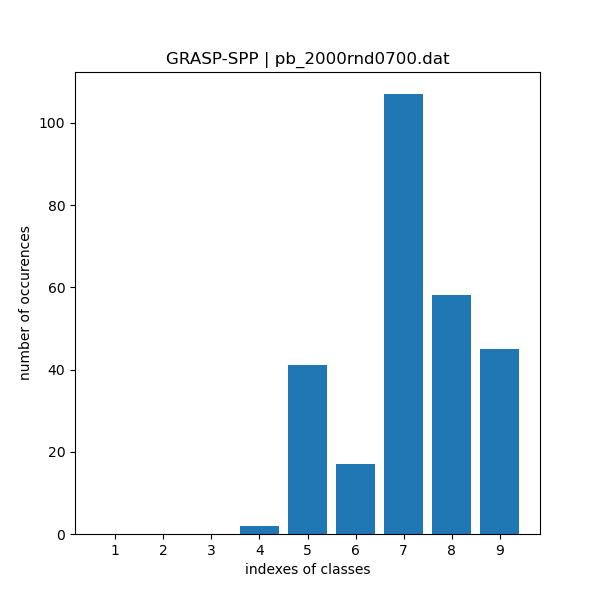
\includegraphics[scale=0.3]{all2000_700.png}
 
 30 runs
\end{column}
\end{columns}

{\tiny
$z$: 
[1703, 1693, 1708, 1692, 1687, 1691, 1713, 1697, 1698, 1689, 1726, 1703, 1693, 1700, 1702, 1686, 1677, 1683, 1689, 1704, 1688, 1689, 1694, 1698, 1689, 1691, 1697, 1700, 1695, 1691]\vspace{1mm}\\
$\Delta$(\%): 
[6.342, 6.97, 6.03, 7.033, 7.35, 7.096, 5.721, 6.718, 6.655, 7.223, 4.925, 6.342, 6.97, 6.529, 6.404, 7.414, 7.99, 7.605, 7.223, 6.279, 7.287, 7.223, 6.907, 6.655, 7.223, 7.096, 6.718, 6.529, 6.844, 7.096]\\
}

\end{frame}

% ================================================================
\begin{frame}


\vspace{10mm}

\begin{center}
    

\textbf{Feedback on three topics related to GRASP}

{\small
Xavier GANDIBLEUX\\ Nantes Université -- France
}
\end{center}
\vspace{7mm}

{\scriptsize 

Xavier Gandibleux, David Vancoppenolle, Daniel Tuyttens.
A first making use of GRASP for solving MOCO problems. 
 \textit{MCDM'1998: 14th International Conference on Multiple Criteria Decision Making}. June 8-12 1998, Charlottesville (VA), USA.
 
Hiroyuki Morita, Xavier Gandibleux, and Naoki Katoh. 
Experimental feedback on biobjective permutation scheduling problems solved with a population heuristic. 
\textit{Foundations of Computing and Decision Sciences Journal}. 26(1):23–50, 2001.

Xavier Delorme, Xavier Gandibleux, and Joaquin Rodriguez. 
GRASP for set packing problems.
 \textit{European Journal of Operational Research}, 153(3):564-580, 2004.
 
Xavier Delorme, Xavier Gandibleux, and Fabien Degoutin. 
Evolutionary, constructive and hybrid procedures for the bi-objective set packing problem. 
\textit{European Journal of Operational Research}. 204(2):206–217, July 2010.
 
 Xavier Gandibleux. 
Peek - Shape - Grab: A Methodology in Three Stages for Approximating the Non-dominated Points of Multiobjective Discrete/Combinatorial Optimization Problems with a Multiobjective Metaheuristic. \textit{Lecture Notes in Computer Science}, vol 10173, 221-235. 2017.

}

\end{frame}



% ================================================================
% ================================================================
% ================================================================

\begin{frame}[standout]


\end{frame}

\end{document}



% ================================================================
\begin{frame}{Multi-objective 0-1 linear optimisation problem ($p$-01LP)}

%Computing \textcolor{purple}{$Y_N$} for \\ 
$$
\begin{array}{rcl}
\min \ z(x) & = & Cx\\
\hbox{s.t. }\quad Ax & \leq & b\\
x & \in & \mB^{n}\\
\end{array}
$$
\vspace{-3mm}
\noindent 
where
%\vspace{-2mm}
%\vfill

\begin{itemize}
    \item $A \in \mR^{m \times n}$ and $b \in \mR^m$; the $m$ constraints $A_ix \leq b_i$, $i = 1,\ldots,m$
    \item $C \in \mR^{p \times n}$, the $p$ objective function $C_kx$, $k = 1,\ldots,p\ge2$
    \item $x \in \mB^{n}$, the vector of $n$ binary variables $x_j$,  $j = 1,\ldots,n$
    \item $X = \{x \in \mB^{n} \mid Ax\leq b \}\subseteq\mR^n$, the feasible decision space
    \item $Y = \{Cx \mid x \in X\} \subseteq \mR^{p}$, the feasible objective space
\end{itemize}
Its LP-relaxation replaces
\begin{itemize}
    \item $x \in \mB^{n}$ by $x \in {[0,1]}^{n}$ and consequently
    \item $X$, by $\bar{X} = \{x \in {[0,1]}^{n} \mid Ax\leqq b \}$
\end{itemize}
\end{frame}
% ================================================================
\begin{frame}{Nondominated Points $(Y_N)$ and Efficient Solutions $(X_E)$}
\begin{itemize}
\item $Y_N=\{y^*\in Y$: $\not\exists\, y\not= y^*\in Y$ $\mid$ $y_k\leq y^*_k,~\forall k=1,...,p$\}

\item $X_E=\{x^*\in X$: $z(x^*)\in Y_N$\}
\end{itemize}
 			
\vspace{3mm}

\begin{center}
\only<1>{\includegraphics[scale=0.4]{ensBornants1.png}}
\end{center}
\end{frame}
% ================================================================
\begin{frame}{Lower ($L$) and Upper Bound ($U$) sets}

\only<1>{
An \blue{upper bound set} for $Y' \subset Y_N$ is a subset $U \subset \mR^p$ such that
\begin{itemize}
\item For each $y \in Y'$ there is some $u \in U$ such that $y \leq u$
\item There is no pair $(y,u) \in Y'\times U$ such that $u$ dominates $y$
\end{itemize}
}
\vspace{1mm}
\begin{center}
\only<1>{\includegraphics[scale=0.4]{ensBornants6.png}}
\end{center}
\vspace{1mm}
\begin{columns}
\begin{column}{0.05\textwidth}
\end{column}
\begin{column}{0.95\textwidth}
\tiny{Matthias Ehrgott and Xavier Gandibleux\\   
Bounds and Bound Sets for Biobjective Combinatorial Optimization Problems\\ 
\textit{Lecture Notes in Economics and Mathematical Systems}, (2001)
\medskip

Matthias Ehrgott and Xavier Gandibleux\\
Bound sets for biobjective combinatorial optimization problems\\
\textit{Computers \& Operations Research}, (2007)
}
\end{column}
\end{columns}
\end{frame}
% ================================================================
\begin{frame}{Multi-Objective Primal Math-Heuristic}
To compute an upper bound set $U$ well representative of $Y_N$, and \red{not} necessary a close approximation of \red{all} $y\in Y_N$, which is a difference with the existing literature.
\vspace{5mm}


The main characteristics: \vspace{-2mm}
\begin{itemize}
    \item Generic designed for any $p$-01LP with $p\ge 2$ 
    \item Easy to implement only MIP solver is needed
\end{itemize}
\vspace{5mm}

The proposed matheuristic is called \red{Gravity Machine}
\end{frame}
% ================================================================
\begin{frame}{Summary}

Our goal:\vspace{-2mm}
\begin{itemize}
    \item[]  \blue{to tighten $L$ and $U$ over $Y_N$ in order to prune as early as possible useless nodes in a branch-and-bound algorithm}
\end{itemize}
\vspace{2mm}

The proposed algorithm:\vspace{-2mm}
\begin{itemize}
    \item[]  \blue{devoted to the upper bound set $U$}
\end{itemize}
\vspace{2mm}

The desirable characteristic: \vspace{-2mm}
\begin{itemize}
    \item[] \blue{$U$ well representative of $Y_N$, and not necessary a close approximation of all $y\in Y_N$, which is a difference with the existing literature}    
\end{itemize}

\end{frame}
% ================================================================
\begin{frame}{Context: $p$-01LP $\rightarrow$ $2$-SPA}

The bi-objective set partitioning problem ($2$-SPA) as benchmark:
\vspace{5mm}
$$
\begin{array}{rcl}
\min \ z(x) & = & Cx\\
\hbox{s/t }\quad  \blue{Ax} & \blue{=} & \blue{1}\\
x & \in & \mB^{n}\\
\end{array}
$$
\vspace{-3mm}
where
\begin{center}
    \quad $C \in \mZ^{p \times n}$ \\
    \quad $\blue{A \in \mB^{m \times n}}$
\end{center}
\pause

\vspace{5mm}
\textcolor{purple}{$Y_N$} computed with the \texttt{vOptGeneric.jl} package of vOptSolver

\vspace{3.5mm}
\begin{columns}
\begin{column}{0.05\textwidth}
\end{column}
\begin{column}{0.95\textwidth}
\tiny{Xavier Gandibleux, Gauthier Soleilhac, Anthony Przybylski, and Stefan Ruzika\\
vOptSolver: an open source software environment for multiobjective mathematical optimization.\\
IFORS2017: 21st Conf. of the Int. Federation of Operational Research Societies. July 17-21, 2017. Quebec City (Canada).\medskip \\

vOptSolver: Solver of multiobjective linear optimization problems. \\  \url{https://github.com/vOptSolver}
}
\end{column}
\end{columns}
\vspace{1mm}

\end{frame}
% ================================================================
% ================================================================
\begin{frame}{Context of multi-objective branch and bound}

Computing \textcolor{purple}{$Y_N$} with a \textbf{MO branch and bound} algorithm: \\
\vspace{1mm}

an implicit enumeration principle viewed as a tree search. 
\vspace{3.5mm}
\begin{columns}
\begin{column}{0.05\textwidth}
\end{column}
\begin{column}{0.95\textwidth}
\tiny{Anthony Przybylski and Xavier Gandibleux. \\
Multi-objective branch and bound. \\
\textit{European Journal of Operational Research} 260, 3 (2017), 856–872.
}
\end{column}
\end{columns}

\vspace{5mm}

\end{frame}
% ================================================================

% ================================================================
% ================================================================
% ================================================================

\begin{frame}[standout]
%\section{1. Introduction}
Feasibility Pump
%General Primal Heuristics\vspace{3mm}\\
%{\small
%from ``Feasibility Pump'' to ...\\
%}

\end{frame}

% ================================================================
\begin{frame}{Feasibility Pump}

A primal heuristic 

\begin{itemize}
    \item introduced in 2005 for computing a feasible solution of single-objective integer linear programs
    \item integrated in several MIP solvers such as GLPK, Gurobi, and CPLEX
    \item adapted in 2019 for MOP as competitor to NSGA-II (Deb et al. 2002), and Multidirectional Local Search (Tricoire 2012)
\end{itemize}
\vspace{5mm}

\begin{columns}
\begin{column}{0.05\textwidth}
\end{column}
\begin{column}{0.95\textwidth}
\tiny{Matteo Fischetti, Fred Glover, and Andrea Lodi.\\
The feasibility pump. \\
\textit{Mathematical Programming} 104(1):91–104, Sep 2005.
\medskip

Timo Berthold, Andrea Lodi, and Domenico Salvagnin.\\
Ten years of feasibility pump, and counting. \\
\textit{EURO Journal on Computational Optimization}, 7, 1–14 (2019).
\medskip

Aritra Pal and Hadi Charkhgard.\\
A Feasibility Pump and Local Search Based Heuristic for Bi-Objective Pure Integer Linear Programming. \\
\textit{INFORMS Journal on Computing} 31, 1 (2019), 115–133.
}
\end{column}
\end{columns}


\end{frame}

% ================================================================
\begin{frame}{Feasibility Pump (Fischetti et al. 2005)}
%\setbeamercovered{transparent}

\vspace{2mm}
\begin{columns}
\begin{column}{0.5\textwidth}

$\bullet$ \blue{Initial solution:}\\ 
$\overline{x}^0 \in \overline{X}$, e.g. $\overline{x}^0 \coloneqq \argmin\{c^T x : x \in \overline{X} \}$\\
\vspace{3mm}

\uncover<2->{
$\bullet$ Two sequences of solutions:\\ 
1) \orange{binary:} $\tilde{x}^{t} \in \mB^n$, $t\ge0$\\  
{\footnotesize
\begin{itemize}
    \item[] by a rounding procedure from $\overline{x}^{t}$
\end{itemize}
}
}
\vspace{2mm}
\uncover<3->{
2) \red{fractional:} $\overline{x}^{t}\in \overline{X}$, $t>0$\\
{\footnotesize
\begin{itemize}
    \item[] optimal solution of the projection problem\\
    \item[] $\overline{x}^{t+1}$ is generated as the closest feasible LP solution with  $\tilde{x}^{t}$
\end{itemize}
}
}
\vspace{2mm}

\uncover<4->{
$\bullet$ Cycles: 
$(\tilde{x}^{t}$, $\tilde{x}^{t'})$, $t'>t$ repeated \\
$\rightarrow$ \textsc{perturbSolution} on $\tilde{x}^{t'}$
}
\end{column}
%
\begin{column}{0.6\textwidth}
  \centering
    \vspace{5mm}
  $\overline{X} = \{x \in \mC^n: Ax\leqq b \}$
    \vspace{3mm}
    
  \only<1>{\includegraphics[width=\linewidth]{FP0.png}}  
  \only<2>{\includegraphics[width=\linewidth]{FP1.png}}    
  \only<3-4>{\includegraphics[width=\linewidth]{FP2.png}}
  \only<5>{\includegraphics[width=\linewidth]{FP3.png}} 
\end{column}
\end{columns}
\vspace{3mm}

\uncover<5->{
\hspace{-7mm}$\bullet$ Stopping conditions: \green{feasible solution} or maxTime limit reached
}

\end{frame}

% ================================================================
\begin{frame}{Feasibility Pump (2005): observation}% (\only<1-2>{1/2}\only<3-4>{2/2})}

\only<1-2>{\vspace{-2mm}~\\ E.g. for instance \texttt{sppnw06}:}
%\only<3-4>{~\vspace{-2mm}\\ E.g. for instance \texttt{sppnw24}:}
\vspace{-5mm}
\begin{center}
%\only<1>{\includegraphics[scale=0.34]{ensBornants1.png}}
\only<1>{\includegraphics[scale=0.25]{FPsppnw06generator16.png}}
\only<2>{\includegraphics[scale=0.25]{FPsppnw06allgenerators.png}}
%\only<3>{\includegraphics[scale=0.25]{FPsppnw24generator16.png}}
%\only<4>{\includegraphics[scale=0.25]{FPsppnw24allgenerators.png}}
\end{center}
%\only<2>{\vspace{-10mm}~\\ Negative result!}
%\only<4>{~\vspace{-5mm}\\ Positive result!}
\end{frame}


% ================================================================
% ================================================================
% ================================================================

\begin{frame}[standout]
%\section{1. Introduction}
Gravity Machine
%General Primal Heuristics\vspace{3mm}\\
%{\small
%...to ``Gravity Machine'' \\
%}

\end{frame}

% ================================================================
\begin{frame}{Gravity Machine}
\vspace{2mm}
\only<1>{\textbf{1/4: A set of generators ($\bar{x}^{k}$, $\bar{y}^{k}$) with $\bar{y}^{k} \coloneqq z(\bar{x}^{k})$:}}
\only<2>{\textbf{2/4: A cone open to the search area in objective space:}}
\only<3>{\textbf{3/4: Alternance of rounding/projecting operations:}}
\only<4>{\textbf{4/4: A cone open to the lower bound set in objective space:}}
\vspace{3mm}
\begin{center}
%\only<1>{\includegraphics[scale=0.34]{ensBornants1.png}}
\only<1>{\includegraphics[scale=0.4]{GMprincipe2a.png}}
\only<2>{\includegraphics[scale=0.4]{GMprincipe2b.png}}
\only<3>{\includegraphics[scale=0.4]{GMprincipe2c.png}}
\only<4>{\includegraphics[scale=0.4]{GMprincipet.png}}

\only<1>{$\epsilon$-constraint LP resolutions \vspace{5mm}}
\only<2>{Hard-constraints over $\bar{y}^{k,t}, t=0$ \vspace{5mm}}
\only<3>{ $\tilde{x}^{k,t}$, $H$, cycle  $\leftarrow$ \textsc{roundingSolution($\bar{x}^{k,t},\ k, \ H$)}\\ and \\ $\bar{x}^{k,t+1} \coloneqq  \argmin \{\Delta(x,\tilde{x}^{k,t}), x\in \overline{X}\}, t\ge 0$ \vspace{1mm}}
\only<4>{Soft-constraints over $\bar{y}^{k,t}, t>0$ \vspace{5mm}}
%\vspace{5mm}
\end{center}

\end{frame}

% ================================================================
\begin{frame}{Gravity Machine: outline of the algorithm}
\begin{center}
\includegraphics[scale=0.3]{algoGM.png}
\end{center}
\end{frame}

% ================================================================
\begin{frame}{Gravity Machine: observation}% (\only<1-2>{1/2}\only<3-4>{2/2})}

\only<1-2>{\vspace{-2mm}~\\ E.g. for instance \texttt{sppnw06}:}
%\only<3-4>{~\vspace{-2mm}\\ E.g. for instance \texttt{sppnw24}:}
\vspace{-2mm}
\begin{center}
%\only<1>{\includegraphics[scale=0.34]{ensBornants1.png}}
\only<1>{\includegraphics[scale=0.25]{GMsppnw06generator16.png}}
\only<2>{\includegraphics[scale=0.25]{GMsppnw06allgenerators.png}}
%\only<3>{\includegraphics[scale=0.25]{GMsppnw24generator16.png}}
%\only<4>{\includegraphics[scale=0.25]{GMsppnw24allgenerators.png}}
\end{center}

\end{frame}

% ================================================================
% ================================================================
% ================================================================

\begin{frame}[standout]
%\section{1. Introduction}
Numerical experiments\vspace{3mm}

\end{frame}

% ================================================================
\begin{frame}{Environment}

Program: \vspace{-3mm}
\begin{itemize}
    \item Algorithm coded in Julia language (1.6) 
    \item Use the algebraic modeling language JuMP (0.21.8) + GLPK (4.65)
\end{itemize}

Numerical instances:\vspace{-3mm}
\begin{itemize}
    \item 44 instances from the OR-library\\
    {\small \url{http://people.brunel.ac.uk/~mastjjb/jeb/orlib/sppinfo.html}}
    \item Second objectives have been generated as follows:\\
    $c^2 \coloneqq$ \texttt{randomShuffle}($c^1$)
    \item Available on the \texttt{vOptLib} (1998-):\\
    {\small \url{https://github.com/vOptSolver/vOptLib/tree/master/SPA}}
\end{itemize}

Computer:\vspace{-3mm}
\begin{itemize}
    \item Intel(R) Core(TM) i7-10870H processor running at 2,20 GHz 
    \item 16 Go of RAM DDR4
\end{itemize}

\end{frame}

% ================================================================
\begin{frame}{Quality measure}

The exclusive hypervolume contribution of solutions:
\medskip

\begin{center}
      \includegraphics[scale=0.4]{GMquality.png}
\end{center}

$$ r= \frac{A_{U}}{A_{Y_N}}$$
\end{frame}

% ================================================================
\begin{frame}{Observing a single run}

Parameters:\vspace{-2mm}
\begin{itemize}
    \item $n_L=30$
    \item \texttt{maxTrial}$\ =5$
    \item \texttt{maxTime}$\ =\infty$.  
\end{itemize}


Measures:\vspace{-0mm}
\begin{itemize}
    \item $r$ the quality measure of $U$
%    \item $\#U$, number of solutions detected
    \item CPUt (sec),
\end{itemize}

Discussion:\vspace{-0mm}
\begin{itemize}
    \item Feasibility pump$^*$ (FP)
    \item Gravity Machine (GM)
%    \item Feasibility Pump and Local Search Based Heuristic (FPBH) 

\end{itemize}

\end{frame}

% ================================================================
\begin{frame}{Measures: top / ratio (\%); bottom / CPUt (s)}

%\begin{center}
      \hspace{-5mm}\includegraphics[scale=0.34]{ratioFPGM.png}
      
      \only<1>{\hspace{-5mm}\includegraphics[scale=0.34]{CPUtFPGM.png}}  
      \only<2>{\hspace{-5mm}\includegraphics[scale=0.34]{CPUtFPGMzoom.png}}        
%\end{center}
\end{frame}

% ================================================================
\begin{frame}{Analysis}

\sethlcolor{green}

\begin{columns}
\begin{column}{0.33\textwidth}
Ratio
\medskip


$
\begin{array}{c|c}
   \hline
   best & /44 \\
   \hline
   \hline
   FP  & 16 \ (36.4\%)  \\
   \textbf{\green{GM}}  & 21 \ (47.6\%) \\
   =   & 07 \ (16.0\%) \\
   \hline
\end{array}
$
\end{column}
\begin{column}{0.33\textwidth}
CPUt
\medskip


$
\begin{array}{c|c}
   \hline
   best & /44 \\
   \hline
   \hline
   \mathbf{\green{FP}}  & 27 \ (61.5\%)  \\
   GM  & 15 \ (34.0\%) \\
   =   & 02 \ (04.5\%) \\
   \hline
\end{array}
$
\end{column}
\begin{column}{0.33\textwidth}
Ratio \& CPUt
\medskip

$
\begin{array}{c|c}
   \hline
   best & /44 \\
   \hline
   \hline
   FP  & 08 \ (18.2\%)  \\
   GM  & 04 \ (09.1\%) \\
   \textbf{\green{none}} & 32 \ (72.7\%) \\
   \hline
\end{array}
$
\end{column}
\end{columns}
\end{frame}

% ================================================================
\begin{frame}{Conclusion}

\begin{itemize}
    \item easy to explain/understand, few parameters\medskip
    \item first results...and they are encouraging\medskip
    \item many potential search directions from now; e.g.:
    \begin{itemize}
      \item using the objectives during the projection (c.f. Objective FP)    
     % \item using the points $\bar{y}^{k,t}, \tilde{y}^{k,t}$ generated by GM
      \item performing a local search on points belonging to $U$
      \item etc.      \medskip
    \end{itemize}
    \item intensive numerical experiments:    
    \begin{itemize}
     % \item various datasets and $p$-01LP
      \item impact of stochastic components
      \item comparison with metaheuristics
      \item etc.
    \end{itemize}    
%    \item advances around the MO branch-and-xxx:    
%    \begin{itemize}
%      \item general efficient scheme
%      \item shared open-source
%      \item more than two objectives
%      \item etc.
%    \end{itemize}    
    
\end{itemize}
\end{frame}

% ================================================================
% ================================================================
% ================================================================

\begin{frame}[standout]

\large{A primal heuristic to compute an upper bound set for multi-objective 0-1 linear optimisation problems}
\vspace{5mm}

Xavier Gandibleux, Guillaume Gasnier, Saïd Hanafi
\vspace{8mm}

\footnotesize{
The source code (soon):\\ \url{https://github.com/xgandibleux/GravityMachine} \medskip\\
The datasets:\\ \url{https://github.com/vOptSolver/vOptLib/tree/master/SPA}
}

\end{frame}

%\end{document}

% ================================================================
\begin{frame}{RAMOO workshop}

%\begin{center}
      \hspace{-5mm}\includegraphics[scale=0.225]{ramoo.png}
%\end{center}
\end{frame}

% ================================================================
\begin{frame}{$L$ and $U$ bound sets}

\begin{center}
%\only<1>{\includegraphics[scale=0.34]{ensBornants1.png}}
\only<1>{\includegraphics[scale=0.4]{ensBornants3.png}}
\only<2>{\includegraphics[scale=0.4]{ensBornants4.png}}
\only<3>{\includegraphics[scale=0.4]{ensBornants5.png}}
\only<4>{\includegraphics[scale=0.4]{ensBornants6.png}}
%\vspace{5mm}
\end{center}
\end{frame}

% ================================================================
\begin{frame}{Bound sets and pruning pending problems}

\vspace{2mm}
Given $L$ for a pending problem:
\vspace{2mm}

\begin{center}
%\only<1>{\includegraphics[scale=0.34]{ensBornants1.png}}
\only<1>{\includegraphics[scale=0.4]{ensBornants7.png}}
\only<2>{\includegraphics[scale=0.4]{ensBornants8.png}}

\vspace{2mm}
\end{center}
\only<1>{$\Rightarrow$ Pruning condition verified}
\only<2>{$\Rightarrow$ Pruning condition not verified}
\end{frame}

% ================================================================
\begin{frame}{Feasibility Pump (2005): observation (\only<1-2>{1/2}\only<3-4>{2/2})}

\only<1-2>{\vspace{-2mm}~\\ E.g. for instance \texttt{sppnw06}:}
\only<3-4>{~\vspace{-2mm}\\ E.g. for instance \texttt{sppnw24}:}
\vspace{-5mm}
\begin{center}
%\only<1>{\includegraphics[scale=0.34]{ensBornants1.png}}
\only<1>{\includegraphics[scale=0.25]{FPsppnw06generator16.png}}
\only<2>{\includegraphics[scale=0.25]{FPsppnw06allgenerators.png}}
\only<3>{\includegraphics[scale=0.25]{FPsppnw24generator16.png}}
\only<4>{\includegraphics[scale=0.25]{FPsppnw24allgenerators.png}}
\end{center}
\only<2>{\vspace{-10mm}~\\ Negative result!}
\only<4>{~\vspace{-5mm}\\ Positive result!}
\end{frame}

% ================================================================
\begin{frame}{Gravity Machine: observation (\only<1-2>{1/2}\only<3-4>{2/2})}

\only<1-2>{\vspace{-2mm}~\\ E.g. for instance \texttt{sppnw06}:}
\only<3-4>{~\vspace{-2mm}\\ E.g. for instance \texttt{sppnw24}:}
\vspace{-2mm}
\begin{center}
%\only<1>{\includegraphics[scale=0.34]{ensBornants1.png}}
\only<1>{\includegraphics[scale=0.25]{GMsppnw06generator16.png}}
\only<2>{\includegraphics[scale=0.25]{GMsppnw06allgenerators.png}}
\only<3>{\includegraphics[scale=0.25]{GMsppnw24generator16.png}}
\only<4>{\includegraphics[scale=0.25]{GMsppnw24allgenerators.png}}
\end{center}

\end{frame}

% ================================================================
\begin{frame}{Conclusion/discussion}

\begin{itemize}
    \item first results...and they are encouraging
    \item many potential search directions from now; e.g.:
    \begin{itemize}
      \item using the objectives during the projection (c.f. Objective FP)    
      \item using the points $\bar{y}^{k,t}, \tilde{y}^{k,t}$ generated by GM
      \item performing a local search on points belonging to $U$
      \item etc.      
    \end{itemize}
    \item intensive numerical experiments:    
    \begin{itemize}
      \item various datasets and $p$-01LP
      \item impact of stochastic components
      \item comparison with metaheuristics
      \item etc.
    \end{itemize}    
    \item advances around the MO branch-and-xxx:    
    \begin{itemize}
      \item general efficient scheme
      \item shared open-source
      \item more than two objectives
      \item etc.
    \end{itemize}    
    
\end{itemize}
\end{frame}

% ================================================================
\begin{frame}{Global results: top / ratio $r$ (\%); bottom / CPUt (s)}

%\begin{center}
      \hspace{-5mm}\includegraphics[scale=0.34]{ratioFPGMFPBH.png}
      
      \hspace{-5mm}\includegraphics[scale=0.34]{timeFPGMFPBH.png}      
%\end{center}
\end{frame}



\end{document}
